% =====================================================================
%  Anatomía de un LLM — Fase I — Módulo 4
%  Cálculo para el aprendizaje automático
%  Compilar: latexmk -r ../latexmkrc M04-calculo.tex
% =====================================================================
\documentclass[11pt,a4paper,twoside,openany]{book}
\usepackage{../estilo-apuntes}

\newcommand{\ApuntesCurso}{Anatomía de un LLM}
\newcommand{\ApuntesModulo}{Módulo 4}

\hypersetup{pdftitle={Módulo 4. Cálculo para el aprendizaje automático},pdfauthor={Anatomía de un LLM}}

% Notación propia del módulo
\newcommand{\diag}{\operatorname{diag}}
\newcommand{\tr}{\operatorname{tr}}
\newcommand{\Var}{\operatorname{Var}}
\newcommand{\dom}{\operatorname{dom}}
\newcommand{\T}{^{\top}}
\newcommand{\uno}{\mathbf{1}}

\begin{document}
\frontmatter
% ------------------------------------------------------------------ Portada
\begin{titlepage}
\centering
\vspace*{2.5cm}
{\large\scshape Anatomía de un LLM}\par
\vspace{0.4cm}
{\normalsize Fundamentos matemáticos de los modelos de lenguaje}\par
\vspace{2.2cm}
\rule{\textwidth}{0.8pt}\par\vspace{0.5cm}
{\small\scshape Fase I \textperiodcentered\ Fundamentos matemáticos}\par\vspace{0.3cm}
{\Huge\bfseries Módulo 4\par}\vspace{0.3cm}
{\LARGE Cálculo para el aprendizaje automático\par}
\vspace{0.5cm}\rule{\textwidth}{0.4pt}\par
\vspace{1.6cm}
{\large Apuntes del curso}\par
\vfill
{\small Edición de octubre de 2026}\par
\end{titlepage}

% ------------------------------------------------------- Presentación
\raggedbottom
\chapter*{Presentación del módulo}
\addcontentsline{toc}{chapter}{Presentación del módulo}
\markboth{Presentación del módulo}{}

Entrenar un modelo de lenguaje consiste en minimizar una función de pérdida $L(\theta)$ que depende de un vector de parámetros $\theta\in\R^{N}$, con $N$ del orden de $10^{9}$ a $10^{12}$. Todos los métodos de entrenamiento empleados en la práctica se basan en el gradiente $\nabla L(\theta)$: la información local de primer orden que indica cómo varía la pérdida al modificar cada parámetro. Este módulo desarrolla el cálculo diferencial de varias variables necesario para definir, calcular, interpretar y comprobar ese gradiente, y lo aplica a las dos piezas que aparecen en todo Transformer: la capa lineal y la combinación de softmax con entropía cruzada.

\section*{Objetivos}
Al finalizar el módulo, el estudiante debe ser capaz de:
\begin{enumerate}[label=\arabic*.]
  \item definir derivada parcial, diferenciabilidad, gradiente y derivada direccional, y demostrar que el gradiente indica la dirección de máximo ascenso;
  \item enunciar y aplicar la regla de la cadena en forma matricial mediante jacobianos, y explicar por qué el modo inverso (retropropagación) es el adecuado para funciones escalares;
  \item obtener a mano los gradientes de una capa lineal, $\partial L/\partial W=\delta x\T$ y $\partial L/\partial x=W\T\delta$, y el gradiente $p-y$ de la entropía cruzada respecto de los logits;
  \item usar el desarrollo de Taylor de segundo orden y el hessiano para clasificar puntos críticos y analizar la estabilidad del descenso de gradiente;
  \item reconocer funciones convexas mediante sus caracterizaciones de primer y segundo orden, demostrar que la entropía cruzada es convexa en los logits y explicar por qué las redes profundas no lo son;
  \item comprobar numéricamente un gradiente con diferencias centradas, acotando los errores de truncamiento y de redondeo.
\end{enumerate}

\section*{Requisitos previos}
Cálculo diferencial de una variable, incluido el teorema de Taylor con resto de Lagrange. Del módulo~1, la función softmax, la función log-suma-exp y la entropía cruzada (tema~4 y tema~5). Del módulo~2, el producto escalar, la norma euclídea, la desigualdad de Cauchy--Schwarz y el producto matricial. Del módulo~3, los autovalores de una matriz simétrica y el teorema espectral, que se usan en los temas~4 y~5.

\section*{Organización}
\begin{center}
\begin{tabular}{@{}cll@{}}
\toprule
Tema & Contenido & Fuentes principales \\
\midrule
1 & Derivadas parciales y gradiente & \cite{mit1802}, \cite{mml}, \cite{d2l} \\
2 & Regla de la cadena y jacobiano & \cite{mml}, \cite{mit1802}, \cite{gbc} \\
3 & Derivadas matriciales: capa lineal y softmax & \cite{mml}, \cite{cs224n}, \cite{cookbook} \\
4 & Taylor, hessiano y puntos críticos & \cite{mml}, \cite{gbc}, \cite{mit1802} \\
5 & Convexidad & \cite{bv}, \cite{ee364a} \\
6 & Diferenciación numérica y comprobación de gradientes & \cite{gbc}, \cite{cs231n} \\
\bottomrule
\end{tabular}
\end{center}

Cada tema termina con una lista de lecturas y con ejercicios graduados en tres niveles: $\star$ comprensión, $\star\star$ cálculo y $\star\star\star$ demostración. Los ejercicios marcados con \emph{Fuente} están adaptados de cursos y libros de texto universitarios; el enunciado se ha redactado de nuevo y, en algunos casos, se han cambiado los datos para que puedan resolverse a mano. Las soluciones completas, paso a paso, están en el \cref{ap:soluciones}.

\section*{Sobre las fuentes}
El texto es de redacción propia. El orden de los temas sigue el capítulo~5 de Deisenroth, Faisal y Ong~\cite{mml}, desde las derivadas parciales hasta la retropropagación y el desarrollo de Taylor multivariable; la intuición geométrica del gradiente y el criterio del hessiano siguen las clases~7 a~11 del curso 18.02 del MIT~\cite{mit1802}. La convexidad se trata como en los capítulos~3 y~4 de Boyd y Vandenberghe~\cite{bv}, texto del curso EE364a de Stanford~\cite{ee364a}, y el análisis numérico del gradiente y del hessiano, como en el capítulo~4 de Goodfellow, Bengio y Courville~\cite{gbc}. Los gradientes de la capa de salida siguen la tarea~2 del curso CS224N de Stanford~\cite{cs224n}, y la comprobación de gradientes, las notas del curso CS231n~\cite{cs231n}.

Se adopta un convenio distinto del de~\cite{mml}: allí el gradiente de una función escalar es un vector fila (un jacobiano $1\times n$); aquí es un vector columna, $\nabla f=J_f\T$, como en~\cite{bv} y~\cite{gbc}. Con este convenio, el gradiente respecto de una matriz tiene la misma forma que la matriz.

\section*{Notación}
\begin{center}
\begin{tabular}{@{}ll@{}}
\toprule
Símbolo & Significado \\
\midrule
$x=(x_1,\dots,x_n)\T\in\R^{n}$ & vector columna; $e_i$ es el $i$-ésimo vector canónico \\
$\uno=(1,\dots,1)\T$ & vector de unos \\
$\mathbb{I}[\cdot]$ & indicador: vale 1 si la condición se cumple y 0 en caso contrario \\
$\partial f/\partial x_i$, $\nabla f(x)$ & derivada parcial y gradiente (vector columna) \\
$D_u f(x)$ & derivada direccional en la dirección unitaria $u$ \\
$J_g(x)\in\R^{m\times n}$ & jacobiano de $g\colon\R^{n}\to\R^{m}$, $(J_g)_{ji}=\partial g_j/\partial x_i$ \\
$H_f(x)$, $\nabla^{2}f(x)$ & hessiano, $(H_f)_{ij}=\partial^{2}f/\partial x_i\partial x_j$ \\
$A\succeq 0$, $A\succ 0$ & $A$ simétrica semidefinida o definida positiva \\
$\lambda_{\min}(A)$, $\lambda_{\max}(A)$ & menor y mayor autovalor de una matriz simétrica \\
$\langle A,B\rangle=\tr(A\T B)$ & producto escalar de Frobenius de matrices \\
$z\in\R^{K}$, $p=\softmax(z)$, $y$ & logits, probabilidades y vector \emph{one-hot} del token correcto \\
$\delta=\partial L/\partial y$ & señal de error que llega a la salida de una capa \\
$\eta>0$ & tasa de aprendizaje \\
$\varepsilon_{\text{máq}}$ & épsilon de la máquina (unidad de redondeo) \\
$o(\cdot)$, $O(\cdot)$ & símbolos de Landau \\
\bottomrule
\end{tabular}
\end{center}

\tableofcontents
\flushbottom

\mainmatter
% =====================================================================
\chapter{Derivadas parciales y gradiente}
\label{tema:1}
% =====================================================================

La pérdida de un modelo de lenguaje es una función escalar de muchas variables. Este tema define las derivadas parciales y la diferenciabilidad, introduce el gradiente y la derivada direccional, y demuestra que el gradiente señala la dirección de máximo ascenso, que es el fundamento del descenso de gradiente. Se siguen las clases~7, 10 y~11 del curso 18.02 del MIT~\cite{mit1802}, la §5.2 de~\cite{mml} y la §2.4 de~\cite{d2l}.

\section{Derivadas parciales}

Sea $U\subseteq\R^{n}$ un abierto y $f\colon U\to\R$. Para estudiar cómo varía $f$ cerca de un punto, se empieza por moverse en una sola coordenada.

\begin{definicion}[Derivada parcial]\label{def:parcial}
La \emph{derivada parcial} de $f$ respecto de $x_i$ en el punto $x\in U$ es
\[
\frac{\partial f}{\partial x_i}(x)=\lim_{h\to 0}\frac{f(x+h\,e_i)-f(x)}{h},
\]
si el límite existe. Equivale a derivar $f$ como función de una sola variable $x_i$, tratando las demás como constantes.
\end{definicion}

\begin{ejemplo}\label{ej:parciales}
Sea $f(x,y)=x^{2}y+3y$. Con $y$ fija, $\partial f/\partial x=2xy$; con $x$ fija, $\partial f/\partial y=x^{2}+3$. En el punto $(2,1)$, donde $f(2,1)=7$, se obtiene $\partial f/\partial x=4$ y $\partial f/\partial y=7$: al aumentar ligeramente $x$, la función crece a razón de~4 unidades por unidad de $x$; al aumentar $y$, a razón de~7.
\end{ejemplo}

\begin{observacion}[Conexión con los LLM]
Si $L(\theta)$ es la pérdida de entropía cruzada de un modelo con parámetros $\theta_1,\dots,\theta_N$, la parcial $\partial L/\partial\theta_i$ mide cuánto aumenta la pérdida, a primer orden, al aumentar el parámetro $\theta_i$ con los demás fijos. Cada paso de entrenamiento calcula las $N$ parciales a la vez.
\end{observacion}

\section{Diferenciabilidad y gradiente}

La existencia de las derivadas parciales no basta para que $f$ se comporte bien cerca de $x$: las parciales solo exploran las direcciones de los ejes. La noción adecuada exige que $f$ admita una buena aproximación lineal en todas las direcciones a la vez~\cite[§5.2]{mml}.

\begin{definicion}[Diferenciabilidad y gradiente]\label{def:diferenciable}
La función $f$ es \emph{diferenciable} en $x\in U$ si existe un vector $g\in\R^{n}$ tal que
\[
f(x+h)=f(x)+g\T h+o(\norm{h})\qquad\text{cuando } h\to 0,
\]
es decir, $\lim_{h\to 0}\bigl(f(x+h)-f(x)-g\T h\bigr)/\norm{h}=0$. El vector $g$ se llama \emph{gradiente} de $f$ en $x$ y se escribe $\nabla f(x)$. La función afín $h\mapsto f(x)+\nabla f(x)\T h$ es la \emph{aproximación lineal} (o de primer orden) de $f$ en $x$.
\end{definicion}

\begin{proposicion}\label{prop:grad-parciales}
Si $f$ es diferenciable en $x$, existen todas las parciales en $x$ y
\[
\nabla f(x)=\Bigl(\frac{\partial f}{\partial x_1}(x),\dots,\frac{\partial f}{\partial x_n}(x)\Bigr)\T.
\]
En particular, el gradiente es único.
\end{proposicion}

\begin{proof}
Sea $g$ un vector como en la \cref{def:diferenciable}. Tomando $h=t\,e_i$ con $t\to 0$, se tiene $\norm{h}=\abs{t}$ y $g\T h=t\,g_i$, luego
\[
\frac{f(x+t\,e_i)-f(x)}{t}-g_i=\frac{f(x+t\,e_i)-f(x)-g\T h}{t}\longrightarrow 0,
\]
porque el cociente por $t$ difiere del cociente por $\abs{t}$ solo en el signo. Así, $\partial f/\partial x_i(x)$ existe y vale $g_i$. Como las parciales están determinadas por $f$, también lo está $g$.
\end{proof}

El gradiente tiene la misma forma que la variable: si $x\in\R^{n}$, entonces $\nabla f(x)\in\R^{n}$. En el \cref{ej:parciales}, $\nabla f(2,1)=(4,7)\T$. Para un LLM, el gradiente de la pérdida tiene tantas componentes como parámetros.

\begin{teorema}[Condición suficiente de diferenciabilidad]\label{teo:C1}
Si todas las derivadas parciales de $f$ existen en un entorno de $x$ y son continuas en $x$, entonces $f$ es diferenciable en $x$. En particular, toda $f\in C^{1}(U)$ es diferenciable en todo punto de $U$.
\end{teorema}

La demostración, estándar en los cursos de cálculo de varias variables, aplica el teorema del valor medio en cada coordenada por separado y se omite aquí. Las funciones que se usan para construir una red (polinomios, exponenciales, logaritmos, cocientes con denominador no nulo y sus composiciones) son de clase $C^{\infty}$ en su dominio. La excepción habitual es la función ReLU, $\max(0,t)$, que no es derivable en $t=0$; el \cref{tema:6} vuelve sobre ella.

\begin{observacion}[Parciales sin diferenciabilidad]
Sea $f(x,y)=xy/(x^{2}+y^{2})$ si $(x,y)\ne(0,0)$ y $f(0,0)=0$. Como $f$ se anula sobre los dos ejes, $\partial f/\partial x(0,0)=\partial f/\partial y(0,0)=0$. Sin embargo, $f(t,t)=1/2$ para todo $t\ne 0$, de modo que $f$ ni siquiera es continua en el origen y, por tanto, no es diferenciable allí. Las parciales existen, pero no son continuas en $(0,0)$.
\end{observacion}

\section{Derivada direccional}

\begin{definicion}[Derivada direccional]\label{def:direccional}
Sea $u\in\R^{n}$ con $\norm{u}=1$. La \emph{derivada direccional} de $f$ en $x$ en la dirección $u$ es
\[
D_u f(x)=\lim_{t\to 0}\frac{f(x+t\,u)-f(x)}{t}.
\]
Las derivadas parciales son las derivadas direccionales en las direcciones $e_1,\dots,e_n$.
\end{definicion}

\begin{proposicion}\label{prop:direccional}
Si $f$ es diferenciable en $x$, entonces $D_u f(x)=\nabla f(x)\T u$ para todo $u$ unitario.
\end{proposicion}

\begin{proof}
Con $h=t\,u$ se tiene $\norm{h}=\abs{t}$. Por la \cref{def:diferenciable}, $f(x+t\,u)-f(x)=t\,\nabla f(x)\T u+o(\abs{t})$. Dividiendo por $t$ y haciendo $t\to 0$ se obtiene el enunciado.
\end{proof}

\begin{ejemplo}\label{ej:direccional}
Con la función del \cref{ej:parciales} y $u=(3/5,\,4/5)\T$, que es unitario, $D_u f(2,1)=4\cdot 0{,}6+7\cdot 0{,}8=8$. Se verá a continuación que ninguna dirección supera $\norm{\nabla f(2,1)}=\sqrt{65}\approx 8{,}062$.
\end{ejemplo}

\section{La dirección de máximo ascenso}

\begin{teorema}[Máximo ascenso]\label{teo:max-ascenso}
Sea $f$ diferenciable en $x$ con $\nabla f(x)\ne 0$. Para todo $u$ unitario,
\[
-\norm{\nabla f(x)}\le D_u f(x)\le\norm{\nabla f(x)}.
\]
La cota superior se alcanza únicamente en $u^{*}=\nabla f(x)/\norm{\nabla f(x)}$ y la inferior únicamente en $-u^{*}$.
\end{teorema}

\begin{proof}
Por la \cref{prop:direccional} y la desigualdad de Cauchy--Schwarz (módulo~2),
\[
\abs{D_u f(x)}=\abs{\nabla f(x)\T u}\le\norm{\nabla f(x)}\,\norm{u}=\norm{\nabla f(x)}.
\]
La igualdad en Cauchy--Schwarz se da si y solo si $u$ es proporcional a $\nabla f(x)$; al ser $u$ unitario, $u=\pm u^{*}$. Sustituyendo, $\nabla f(x)\T u^{*}=\norm{\nabla f(x)}^{2}/\norm{\nabla f(x)}=\norm{\nabla f(x)}$, y con $-u^{*}$ se obtiene el valor opuesto.
\end{proof}

Así, $\nabla f(x)$ apunta en la dirección en la que $f$ crece más deprisa, su norma es esa tasa máxima de crecimiento y $-\nabla f(x)$ es la dirección de \emph{máximo descenso}.

\begin{lema}[Derivada a lo largo de una curva]\label{lem:curva}
Sea $r\colon(a,b)\to U$ derivable en $t_0$ y $f$ diferenciable en $r(t_0)$. Entonces $t\mapsto f(r(t))$ es derivable en $t_0$ y
\[
\frac{d}{dt}f(r(t))\Big|_{t=t_0}=\nabla f(r(t_0))\T r'(t_0).
\]
\end{lema}

\begin{proof}
Sea $x=r(t_0)$ y $h(s)=r(t_0+s)-x$, de modo que $h(s)=s\,r'(t_0)+o(s)$ y $\norm{h(s)}=O(\abs{s})$. Por la \cref{def:diferenciable}, $f(r(t_0+s))-f(x)=\nabla f(x)\T h(s)+o(\norm{h(s)})=s\,\nabla f(x)\T r'(t_0)+o(s)$. Dividiendo por $s$ y haciendo $s\to 0$ se obtiene el enunciado.
\end{proof}

El \cref{lem:curva} es un caso particular de la regla de la cadena, que se estudia en general en el \cref{tema:2}.

\begin{corolario}[Gradiente y conjuntos de nivel]\label{cor:nivel}
Sea $r$ una curva derivable contenida en un conjunto de nivel de $f$, es decir, $f(r(t))=c$ para todo $t$. Entonces $\nabla f(r(t))\T r'(t)=0$: el gradiente es ortogonal a la recta tangente a la curva de nivel.
\end{corolario}

\begin{proof}
La función $t\mapsto f(r(t))$ es constante; su derivada es nula y, por el \cref{lem:curva}, es igual a $\nabla f(r(t))\T r'(t)$.
\end{proof}

\begin{figure}[h]
\centering
\begin{tikzpicture}[scale=1.45,font=\small]
  \draw[->,gray] (-2.4,0) -- (2.8,0) node[right] {$x$};
  \draw[->,gray] (0,-1.4) -- (0,2.3) node[above] {$y$};
  \foreach \c in {1,2.5,4} {
    \draw[thick] (0,0) ellipse ({sqrt(\c)} and {sqrt(\c/3)});
  }
  \draw[dashed,gray!60!black] (-0.65,1.55) -- (2.35,0.55);
  \draw[->,>={Stealth[length=2.2mm]},very thick] (1,1) -- (1.33,1.99);
  \node[right] at (1.36,1.95) {$\nabla f(1,1)=(2,6)\T$};
  \fill (1,1) circle (1.4pt);
  \node[below left] at (1,1) {$(1,1)$};
  \node at (-1.75,1.25) {$f=4$};
\end{tikzpicture}
\caption{Curvas de nivel $x^{2}+3y^{2}=c$ para $c=1$; $2{,}5$; $4$. En $(1,1)$ el gradiente (flecha, a escala reducida) es perpendicular a la tangente a la curva $f=4$ (trazo discontinuo), de dirección $(3,-1)\T$.}
\label{fig:nivel}
\end{figure}

\section{Descenso de gradiente}

El \cref{teo:max-ascenso} sugiere un método para minimizar $f$: desplazarse repetidamente en la dirección $-\nabla f$.

\begin{definicion}[Descenso de gradiente]\label{def:dg}
Dado un punto inicial $x_0$ y una \emph{tasa de aprendizaje} $\eta>0$, el \emph{descenso de gradiente} genera la sucesión
\[
x_{k+1}=x_k-\eta\,\nabla f(x_k),\qquad k=0,1,2,\dots
\]
\end{definicion}

\begin{proposicion}[Descenso a primer orden]\label{prop:descenso}
Si $f$ es diferenciable en $x$ y $g=\nabla f(x)\ne 0$, existe $\eta_0>0$ tal que $f(x-\eta g)<f(x)$ para todo $\eta\in(0,\eta_0)$.
\end{proposicion}

\begin{proof}
Por la \cref{def:diferenciable} con $h=-\eta g$, $f(x-\eta g)=f(x)-\eta\norm{g}^{2}+o(\eta)$. Luego $\bigl(f(x-\eta g)-f(x)\bigr)/\eta\to-\norm{g}^{2}<0$ cuando $\eta\to 0^{+}$, y el cociente es negativo para todo $\eta$ suficientemente pequeño.
\end{proof}

La proposición garantiza el descenso solo para pasos pequeños. El tamaño máximo admisible depende de la curvatura de $f$ y se determina en el \cref{tema:4}.

\begin{ejemplo}\label{ej:dg}
Sea $f(x,y)=x^{2}+3y^{2}$, con $\nabla f=(2x,6y)\T$. Desde $(1,1)$, con $\nabla f(1,1)=(2,6)\T$ y $\eta=0{,}1$, el primer paso da $(1,1)-0{,}1\,(2,6)=(0{,}8;\,0{,}4)$, y la función baja de $f(1,1)=4$ a $f(0{,}8;\,0{,}4)=0{,}64+0{,}48=1{,}12$.
\end{ejemplo}

\begin{observacion}[Conexión con los LLM]
El entrenamiento de un modelo de lenguaje aplica la \cref{def:dg} a la pérdida $L(\theta)$, con el gradiente estimado sobre un lote de datos. Los métodos que se usan en la práctica (descenso estocástico, momento, Adam) modifican esta iteración y se estudian en el módulo~7.
\end{observacion}

\begin{observacion}[Relación con la física]
Una partícula en un potencial $U(x)$ sometida a un rozamiento muy fuerte se mueve con velocidad proporcional a la fuerza $-\nabla U$: $\dot x(t)=-\nabla U(x(t))$. Esta ecuación se llama \emph{flujo de gradiente}, y la \cref{def:dg} es su discretización por el método de Euler con paso $\eta$. Añadir un término de ruido da la dinámica de Langevin, que sirve de modelo para el descenso de gradiente estocástico.
\end{observacion}

\begin{lecturas}
\item MIT 18.02~\cite{mit1802}, clase~7 «Level Curves, Partial Derivatives, Tangent Plane» y clase~11 «Gradient, Directional Derivative».
\item Deisenroth, Faisal y Ong~\cite{mml}, §5.2 «Partial Differentiation and Gradients».
\item Zhang \emph{et al.}~\cite{d2l}, §2.4.3 «Partial Derivatives and Gradients».
\item Goodfellow, Bengio y Courville~\cite{gbc}, §4.3 «Gradient-Based Optimization».
\end{lecturas}

\section*{Ejercicios del tema 1}
\addcontentsline{toc}{section}{Ejercicios del tema 1}

\begin{ejercicio}{1}{eje:1-vf}
Justifique si son verdaderas o falsas: (a) el gradiente es perpendicular a las curvas de nivel; (b) $-\nabla f$ es la dirección de máximo descenso; (c) si existen todas las derivadas parciales de $f$ en $x$, entonces $f$ es diferenciable en $x$.
\end{ejercicio}

\begin{ejercicio}{2}{eje:1-gradiente}
Sea $f(x,y)=x^{3}+2xy^{2}$. Calcule $\nabla f(1,2)$, su norma y la derivada direccional en la dirección $(1,1)\T/\sqrt{2}$. Compruebe que esta última no supera la norma del gradiente.
\end{ejercicio}

\begin{ejercicio}{2}{eje:1-d2l}
Sea $f(x)=3x_1^{2}+5e^{x_2}$. Calcule $\nabla f$ en un punto genérico y en $(1,0)$. Halle la derivada direccional en $(1,0)$ en la dirección del vector $(3,4)\T$ y compárela con $\norm{\nabla f(1,0)}$.
\fuente{adaptado de Zhang \emph{et al.}~\cite{d2l}, §2.4, ejercicio~7 (se añaden el punto y la dirección).}
\end{ejercicio}

\begin{ejercicio}{2}{eje:1-norma}
Calcule el gradiente de $f(x)=\norm{x}$ para $x\in\R^{n}\setminus\{0\}$ y evalúelo en $x=(3,4)\T$. Estudie qué ocurre en $x=0$. Relacione el resultado con el recorte de gradientes por norma, que divide un gradiente $g$ por $\norm{g}$ cuando esta supera un umbral.
\fuente{adaptado de Zhang \emph{et al.}~\cite{d2l}, §2.4, ejercicio~8.}
\end{ejercicio}

\begin{ejercicio}{2}{eje:1-mit}
Sea $f(x,y)=x^{3}-3x^{2}+xy-y^{2}+x+y$. En el punto $(1,1/2)$, determine la dirección unitaria en la que la derivada direccional es máxima y su valor, la dirección en la que es mínima y las direcciones en las que es nula.
\fuente{adaptado de MIT 18.02, primavera de 2006~\cite{mit1802}, \emph{Problem Set}~4, segunda parte, problema~5.}
\end{ejercicio}

\begin{ejercicio}{3}{eje:1-minimo}
Sea $f$ diferenciable en $x$ con $\nabla f(x)\ne 0$. Demuestre, sin usar el \cref{teo:max-ascenso}, que el mínimo de $D_u f(x)$ sobre los vectores unitarios vale $-\norm{\nabla f(x)}$ y se alcanza solo en $u=-\nabla f(x)/\norm{\nabla f(x)}$. Deduzca, para $f(x,y)=x^{2}+y^{2}$, que el gradiente es perpendicular a las circunferencias $x^{2}+y^{2}=c$ parametrizándolas como $r(t)=\sqrt{c}\,(\cos t,\sin t)\T$.
\end{ejercicio}

% =====================================================================
\chapter{Regla de la cadena y jacobiano}
\label{tema:2}
% =====================================================================

Una red neuronal es una composición de muchas funciones sencillas, y su pérdida depende de cada parámetro a través de largas cadenas de cálculos intermedios. Este tema generaliza la derivada a funciones con valores vectoriales mediante el jacobiano, demuestra la regla de la cadena en forma matricial y muestra cómo se organiza el cálculo sobre un grafo computacional, en modo directo o en modo inverso. Se sigue~\cite[§5.2, §5.3 y §5.6]{mml}, la clase~10 de~\cite{mit1802} y~\cite[§6.5]{gbc}.

\section{Funciones vectoriales y jacobiano}

\begin{definicion}[Jacobiano]\label{def:jacobiano}
Sea $U\subseteq\R^{n}$ abierto y $g=(g_1,\dots,g_m)\T\colon U\to\R^{m}$. La función $g$ es \emph{diferenciable} en $x$ si existe una matriz $J\in\R^{m\times n}$ tal que
\[
g(x+h)=g(x)+J\,h+o(\norm{h})\qquad\text{cuando } h\to 0.
\]
La matriz $J$ se llama \emph{jacobiano} de $g$ en $x$ y se escribe $J_g(x)$. Aplicando la \cref{prop:grad-parciales} a cada componente, $g$ es diferenciable si y solo si lo es cada $g_j$, y
\[
\bigl(J_g(x)\bigr)_{ji}=\frac{\partial g_j}{\partial x_i}(x),\qquad j=1,\dots,m,\quad i=1,\dots,n.
\]
La fila $j$ de $J_g(x)$ es $\nabla g_j(x)\T$; la columna $i$ es la derivada de $g$ respecto de $x_i$.
\end{definicion}

El jacobiano tiene una fila por cada salida y una columna por cada entrada. Para $m=1$ es una matriz fila y $\nabla f(x)=J_f(x)\T$.

\begin{ejemplo}\label{ej:jac-lineal}
Si $g(x)=Ax+b$ con $A\in\R^{m\times n}$ y $b\in\R^{m}$, entonces $g(x+h)=g(x)+Ah$ exactamente, luego $J_g(x)=A$ en todo punto. El jacobiano de una aplicación afín es su matriz.
\end{ejemplo}

\begin{ejemplo}\label{ej:jac}
Sea $g(x,y)=(xy,\;x^{2}+y)\T$. Entonces
\[
J_g(x,y)=\begin{pmatrix} y & x\\ 2x & 1\end{pmatrix},\qquad J_g(2,1)=\begin{pmatrix} 1 & 2\\ 4 & 1\end{pmatrix}.
\]
\end{ejemplo}

\section{La regla de la cadena}

\begin{teorema}[Regla de la cadena]\label{teo:cadena}
Sean $g\colon U\subseteq\R^{n}\to\R^{m}$ diferenciable en $x$ y $f\colon V\subseteq\R^{m}\to\R^{k}$ diferenciable en $g(x)$, con $g(U)\subseteq V$. Entonces $f\circ g$ es diferenciable en $x$ y
\[
J_{f\circ g}(x)=J_f\bigl(g(x)\bigr)\,J_g(x).
\]
\end{teorema}

\begin{proof}
Sean $A=J_g(x)$, $B=J_f(g(x))$ y $\Delta(h)=g(x+h)-g(x)=Ah+r_1(h)$, con $r_1(h)=o(\norm{h})$. Entonces $\norm{\Delta(h)}\le\norm{A}\,\norm{h}+\norm{r_1(h)}=O(\norm{h})$, donde $\norm{A}$ es la norma de operador. Por la diferenciabilidad de $f$ en $g(x)$,
\[
f\bigl(g(x+h)\bigr)-f\bigl(g(x)\bigr)=B\,\Delta(h)+r_2\bigl(\Delta(h)\bigr)=BA\,h+B\,r_1(h)+r_2\bigl(\Delta(h)\bigr),
\]
con $r_2(v)=o(\norm{v})$. El término $B\,r_1(h)$ es $o(\norm{h})$ porque $\norm{B\,r_1(h)}\le\norm{B}\,\norm{r_1(h)}$. Para el último, si $\Delta(h)\ne 0$ se escribe $\norm{r_2(\Delta)}/\norm{h}=\bigl(\norm{r_2(\Delta)}/\norm{\Delta}\bigr)\bigl(\norm{\Delta}/\norm{h}\bigr)$: el primer factor tiende a~0 porque $\Delta(h)\to 0$, y el segundo está acotado; si $\Delta(h)=0$, el término es nulo. Luego $f\circ g$ es diferenciable en $x$ con jacobiano $BA$.
\end{proof}

\begin{corolario}[Caso escalar]\label{cor:cadena-escalar}
Si $f\colon\R^{m}\to\R$ y $u=g(x)$, entonces
\[
\frac{\partial (f\circ g)}{\partial x_i}(x)=\sum_{j=1}^{m}\frac{\partial f}{\partial u_j}(u)\,\frac{\partial u_j}{\partial x_i}(x),
\qquad\text{es decir,}\qquad
\nabla_x (f\circ g)=J_g(x)\T\,\nabla_u f(u).
\]
\end{corolario}

\begin{proof}
Con $k=1$, el \cref{teo:cadena} da $J_{f\circ g}=\nabla f(u)\T J_g(x)$, una matriz fila cuya entrada $i$ es la suma del enunciado. Trasponiendo se obtiene la forma vectorial.
\end{proof}

La suma del \cref{cor:cadena-escalar} tiene una lectura directa: si $x_i$ influye en $f$ a través de varias variables intermedias $u_j$, su efecto total es la suma de los efectos transmitidos por cada una de ellas.

\begin{ejemplo}\label{ej:cadena}
Sea $f(u,v)=u^{2}v$ y $g$ la del \cref{ej:jac}, en el punto $(x,y)=(2,1)$.
\begin{enumerate}[label=\arabic*.]
  \item Valores intermedios: $u=xy=2$, $v=x^{2}+y=5$, $f=u^{2}v=20$.
  \item Gradiente exterior: $\partial f/\partial u=2uv=20$ y $\partial f/\partial v=u^{2}=4$.
  \item Por el \cref{cor:cadena-escalar},
  \[
  \nabla_{(x,y)}f=J_g(2,1)\T\begin{pmatrix}20\\4\end{pmatrix}=\begin{pmatrix}1&4\\2&1\end{pmatrix}\begin{pmatrix}20\\4\end{pmatrix}=\begin{pmatrix}36\\44\end{pmatrix}.
  \]
\end{enumerate}
Como comprobación, $f(g(x,y))=x^{2}y^{2}(x^{2}+y)=x^{4}y^{2}+x^{2}y^{3}$, cuyas parciales en $(2,1)$ son $4x^{3}y^{2}+2xy^{3}=32+4=36$ y $2x^{4}y+3x^{2}y^{2}=32+12=44$.
\end{ejemplo}

\section{Grafos computacionales}

\begin{definicion}[Grafo computacional]\label{def:grafo}
Un \emph{grafo computacional} es un grafo dirigido acíclico cuyos nodos son variables: los nodos sin predecesores son las entradas, y cada uno de los demás nodos $v$ se calcula como una función diferenciable $v=\phi_v(\text{padres}(v))$ de sus predecesores. Si la salida es un escalar $f$, se llama \emph{adjunto} de un nodo $v$ a $\bar v=\partial f/\partial v$, la derivada de $f$ respecto de $v$ considerando todas las variables posteriores como funciones de $v$~\cite[§6.5.1]{gbc}.
\end{definicion}

\begin{proposicion}[Retropropagación]\label{prop:retro}
En un grafo computacional con salida escalar $f$ se cumple $\bar f=1$ y, para todo nodo $v\neq f$,
\[
\bar v=\sum_{w\,:\,v\in\text{padres}(w)}\bar w\;\frac{\partial\phi_w}{\partial v}.
\]
Por tanto, recorriendo los nodos en orden topológico inverso se obtienen los adjuntos de todas las entradas, es decir, el gradiente de $f$.
\end{proposicion}

\begin{proof}
La variable $v$ influye en $f$ solo a través de los nodos $w$ de los que es padre. Considerando $f$ como función de esos nodos y estos como funciones de $v$, el \cref{cor:cadena-escalar} da la suma del enunciado. En orden topológico inverso, cuando se procesa $v$ ya se conocen todos los $\bar w$ de sus hijos.
\end{proof}

\begin{figure}[h]
\centering
\begin{tikzpicture}[>={Stealth[length=2mm]},font=\small,
  nodo/.style={draw,thick,rounded corners=2pt,minimum width=17mm,minimum height=7mm,align=center},
  adj/.style={->,dashed,gray!70!black}]
  \node[nodo] (x) at (0,1.3) {$x=2$};
  \node[nodo] (y) at (0,-1.3) {$y=1$};
  \node[nodo] (u) at (4,1.3) {$u=xy=2$};
  \node[nodo] (v) at (4,-1.3) {$v=x^{2}+y=5$};
  \node[nodo] (f) at (8,0) {$f=u^{2}v=20$};
  \draw[->,thick] (x) -- (u);
  \draw[->,thick] (y) -- (u);
  \draw[->,thick] (x) -- (v);
  \draw[->,thick] (y) -- (v);
  \draw[->,thick] (u) -- (f);
  \draw[->,thick] (v) -- (f);
  \node[above=1pt of u,gray!30!black] {$\bar u=2uv=20$};
  \node[below=1pt of v,gray!30!black] {$\bar v=u^{2}=4$};
  \node[above=1pt of f,gray!30!black] {$\bar f=1$};
  \node[above=1pt of x,gray!30!black] {$\bar x=\bar u\,y+\bar v\,2x=20+16=36$};
  \node[below=1pt of y,gray!30!black] {$\bar y=\bar u\,x+\bar v\cdot 1=40+4=44$};
\end{tikzpicture}
\caption{Grafo computacional del \cref{ej:cadena}. Dentro de cada nodo figura el valor calculado en el paso hacia delante; junto a él, en gris, el adjunto calculado en el paso hacia atrás con la \cref{prop:retro}. La entrada $x$ recibe contribuciones por dos caminos, que se suman.}
\label{fig:grafo}
\end{figure}

\section{Modo directo y modo inverso}

Sea una composición $F=f_L\circ\dots\circ f_1$, con $f_\ell\colon\R^{d_{\ell-1}}\to\R^{d_\ell}$. Por el \cref{teo:cadena},
\[
J_F=J_L\,J_{L-1}\cdots J_1,\qquad J_\ell\in\R^{d_\ell\times d_{\ell-1}},
\]
con cada $J_\ell$ evaluado en el valor intermedio correspondiente. El producto de matrices es asociativo, pero el coste de calcularlo depende del orden en que se agrupen los factores~\cite[§5.6]{mml}.

\begin{proposicion}[Coste de los dos modos]\label{prop:modos}
Multiplicar una matriz $a\times b$ por otra $b\times c$ requiere $abc$ productos escalares. En consecuencia:
\begin{enumerate}
  \item en \emph{modo directo}, se calcula $J_F v=J_L(\cdots(J_2(J_1 v)))$ para un vector $v\in\R^{d_0}$ con $\sum_\ell d_\ell d_{\ell-1}$ productos; obtener el jacobiano completo exige repetirlo $d_0$ veces, una por columna;
  \item en \emph{modo inverso}, se calcula $w\T J_F=((w\T J_L)J_{L-1})\cdots J_1$ para un vector $w\in\R^{d_L}$ con el mismo número de productos; obtener el jacobiano completo exige repetirlo $d_L$ veces, una por fila.
\end{enumerate}
Si la salida es escalar ($d_L=1$), el gradiente se obtiene con una sola pasada en modo inverso.
\end{proposicion}

\begin{proof}
Cada factor $J_\ell$ aplicado a un vector (por la derecha o por la izquierda) cuesta $d_\ell d_{\ell-1}$ productos, y en cada modo se realizan $L$ de estas operaciones. Con $v=e_i$ se obtiene la columna $i$ de $J_F$, y con $w=e_j$, la fila $j$. Con $d_L=1$, la única fila es $\nabla F\T$.
\end{proof}

La retropropagación de la \cref{prop:retro} es el modo inverso aplicado a un grafo. Su coste es un múltiplo pequeño del coste de evaluar $f$, independiente del número de entradas; por ello la pérdida de un modelo con miles de millones de parámetros puede derivarse con una sola pasada hacia atrás. El precio es la memoria: el paso hacia atrás necesita los valores intermedios del paso hacia delante. La implementación de este mecanismo (diferenciación automática) es el objeto del módulo~10.

\begin{observacion}[Conexión con los LLM]
Un Transformer es un grafo computacional con miles de millones de nodos. Su salida escalar es la pérdida media del lote, y las bibliotecas como PyTorch o JAX registran el grafo durante el paso hacia delante para recorrerlo después en orden inverso. Ninguna de ellas forma explícitamente un jacobiano: solo calculan productos de la forma $w\T J_\ell$.
\end{observacion}

\begin{lecturas}
\item Deisenroth, Faisal y Ong~\cite{mml}, §5.2 (regla de la cadena), §5.3 «Gradients of Vector-Valued Functions» y §5.6 «Backpropagation and Automatic Differentiation».
\item MIT 18.02~\cite{mit1802}, clase~10 «Differentials; Chain Rule».
\item Goodfellow, Bengio y Courville~\cite{gbc}, §6.5.1 «Computational Graphs», §6.5.2 «Chain Rule of Calculus» y §6.5.3 «Recursively Applying the Chain Rule to Obtain Backprop».
\item Zhang \emph{et al.}~\cite{d2l}, §2.4.4 «Chain Rule».
\end{lecturas}

\section*{Ejercicios del tema 2}
\addcontentsline{toc}{section}{Ejercicios del tema 2}

\begin{ejercicio}{1}{eje:2-formas}
Sean $g\colon\R^{5}\to\R^{3}$, $h\colon\R^{3}\to\R^{2}$ y $f\colon\R^{2}\to\R$ diferenciables. Indique la forma de $J_g$, $J_h$, $J_f$ y $J_{f\circ h\circ g}$, y la del gradiente de $f\circ h\circ g$. Compruebe que las dimensiones del producto del \cref{teo:cadena} encajan.
\end{ejercicio}

\begin{ejercicio}{2}{eje:2-producto}
Sea $F(x,y)=(x+y^{2})(x^{2}-y)$. Calcule $\partial F/\partial x$ y $\partial F/\partial y$ en $(1,2)$ con la regla de la cadena, tomando $u=x+y^{2}$ y $v=x^{2}-y$, y compruebe el resultado desarrollando $F$.
\end{ejercicio}

\begin{ejercicio}{2}{eje:2-jacobiano}
Sea $g(x,y)=(x^{2}y,\;3x-y,\;xy)\T$. Escriba $J_g(1,2)$ e indique su forma. Use $J_g\T$ para obtener el gradiente de $s=g_1+g_2+g_3$ en $(1,2)$.
\end{ejercicio}

\begin{ejercicio}{2}{eje:2-d2l}
Sea $w=f(x,y,z)$, donde $x$, $y$ y $z$ son funciones de dos variables $a$ y $b$. (a) Escriba la regla de la cadena para $\partial w/\partial a$ y $\partial w/\partial b$. (b) Aplíquela con $f(x,y,z)=xyz$, $x=a+b$, $y=a-b$, $z=ab$, en $(a,b)=(2,1)$, y compruebe el resultado expresando $w$ directamente en función de $a$ y $b$.
\fuente{adaptado de Zhang \emph{et al.}~\cite{d2l}, §2.4, ejercicio~9 (se añade el caso numérico).}
\end{ejercicio}

\begin{ejercicio}{2}{eje:2-coste}
Sea $F=f_3\circ f_2\circ f_1$ con $f_1\colon\R^{n}\to\R^{d}$, $f_2\colon\R^{d}\to\R^{d}$ y $f_3\colon\R^{d}\to\R$. Cuente los productos escalares necesarios para obtener $\nabla F$ multiplicando los jacobianos (a) de derecha a izquierda, $J_3(J_2J_1)$, y (b) de izquierda a derecha, $(J_3J_2)J_1$. Evalúe ambos con $n=d=1000$.
\end{ejercicio}

\begin{ejercicio}{3}{eje:2-escalar}
Sean $a,b\colon\R^{n}\to\R^{m}$ diferenciables y $s(x)=a(x)\T b(x)$. Demuestre, con el \cref{teo:cadena}, que $\nabla s(x)=J_a(x)\T b(x)+J_b(x)\T a(x)$. Deduzca el gradiente de la forma cuadrática $q(x)=x\T Ax$ para $A\in\R^{n\times n}$ y particularícelo al caso simétrico.
\end{ejercicio}

% =====================================================================
\chapter{Derivadas matriciales: capa lineal y softmax}
\label{tema:3}
% =====================================================================

Casi todo el cómputo del entrenamiento de un modelo de lenguaje consiste en derivar dos tipos de operación: capas lineales y la combinación de softmax con entropía cruzada en la salida. Este tema define el gradiente de una función escalar respecto de una matriz, obtiene los gradientes de la capa lineal, individualmente y por lotes, y deduce el resultado más usado del curso: el gradiente de la entropía cruzada respecto de los logits es $p-y$. Se sigue~\cite[§5.3--§5.5]{mml}, la tarea~2 de~\cite{cs224n} y, como tabla de consulta, \cite{cookbook}.

\section{Gradiente respecto de una matriz}

\begin{definicion}[Gradiente respecto de una matriz]\label{def:grad-matriz}
Sea $L\colon\R^{m\times n}\to\R$. Su \emph{gradiente} en $W$ es la matriz $\nabla_W L=\partial L/\partial W\in\R^{m\times n}$ de entradas
\[
\Bigl(\frac{\partial L}{\partial W}\Bigr)_{ij}=\frac{\partial L}{\partial W_{ij}}.
\]
Equivale a identificar $\R^{m\times n}$ con $\R^{mn}$ y reordenar el gradiente con la forma de $W$.
\end{definicion}

\begin{proposicion}[Aproximación lineal]\label{prop:frobenius}
Si $L$ es diferenciable en $W$, para toda perturbación $E\in\R^{m\times n}$,
\[
L(W+E)=L(W)+\Bigl\langle\frac{\partial L}{\partial W},E\Bigr\rangle+o(\norm{E}),\qquad
\langle A,B\rangle=\sum_{i,j}A_{ij}B_{ij}=\tr(A\T B).
\]
\end{proposicion}

\begin{proof}
Es la \cref{def:diferenciable} en $\R^{mn}$: el término lineal $\nabla L\T h$ es $\sum_{i,j}(\partial L/\partial W_{ij})E_{ij}$. La igualdad $\sum_{i,j}A_{ij}B_{ij}=\tr(A\T B)$ se obtiene desarrollando $(A\T B)_{jj}=\sum_i A_{ij}B_{ij}$ y sumando en $j$.
\end{proof}

La regla práctica que se deriva es que \emph{el gradiente de un escalar respecto de un parámetro tiene la misma forma que el parámetro}. Comprobar las formas es la primera verificación de cualquier fórmula de este tema.

\section{La capa lineal}

\begin{proposicion}[Gradientes de una capa lineal]\label{prop:capa}
Sean $W\in\R^{m\times n}$, $x\in\R^{n}$, $b\in\R^{m}$, $y=Wx+b$ y $L=\ell(y)$ con $\ell\colon\R^{m}\to\R$ diferenciable. Sea $\delta=\nabla_y\ell\in\R^{m}$ la \emph{señal de error} que llega a la salida. Entonces
\[
\frac{\partial L}{\partial W}=\delta\,x\T,\qquad
\frac{\partial L}{\partial b}=\delta,\qquad
\frac{\partial L}{\partial x}=W\T\delta.
\]
\end{proposicion}

\begin{proof}
Como $y_k=\sum_{j}W_{kj}x_j+b_k$, se tiene $\partial y_k/\partial W_{ij}=\mathbb{I}[k=i]\,x_j$: la entrada $W_{ij}$ solo afecta a la salida $y_i$. Por el \cref{cor:cadena-escalar},
\[
\frac{\partial L}{\partial W_{ij}}=\sum_{k}\delta_k\,\frac{\partial y_k}{\partial W_{ij}}=\delta_i\,x_j=(\delta x\T)_{ij}.
\]
Del mismo modo, $\partial y_k/\partial b_i=\mathbb{I}[k=i]$ da $\partial L/\partial b_i=\delta_i$. Por último, $J_y(x)=W$ (\cref{ej:jac-lineal}) y el \cref{cor:cadena-escalar} da $\partial L/\partial x=W\T\delta$.
\end{proof}

Las formas encajan: $\delta x\T$ es $(m\times 1)(1\times n)=m\times n$, como $W$, y $W\T\delta$ es $(n\times m)(m\times 1)=n\times 1$, como $x$. El vector $W\T\delta$ es la señal de error que la capa transmite a la capa anterior.

\begin{ejemplo}\label{ej:capa}
Sean $W=\begin{pmatrix}1&2\\0&1\end{pmatrix}$, $x=(1,-1)\T$, $b=0$, un objetivo $t=(0,1)\T$ y $L=\tfrac12\norm{y-t}^{2}$, de modo que $\delta=y-t$.
\begin{center}\small
\begin{tabular}{@{}lll@{}}
\toprule
Paso & Cálculo & Resultado \\
\midrule
Hacia delante & $y=Wx$ & $(-1,-1)\T$ \\
Pérdida & $\tfrac12\bigl((-1)^{2}+(-2)^{2}\bigr)$ & $2{,}5$ \\
Señal de error & $\delta=y-t$ & $(-1,-2)\T$ \\
Gradiente de $W$ & $\delta x\T$ & $\begin{pmatrix}-1&1\\-2&2\end{pmatrix}$ \\[2mm]
Gradiente de $x$ & $W\T\delta$ & $(-1,-4)\T$ \\
\bottomrule
\end{tabular}
\end{center}
\end{ejemplo}

\begin{corolario}[Capa lineal por lotes]\label{cor:lotes}
Sean $X\in\R^{B\times n}$ una matriz cuyas filas son $B$ ejemplos, $W\in\R^{n\times m}$, $Z=XW\in\R^{B\times m}$ y $L=\ell(Z)$ con $\Delta=\partial L/\partial Z\in\R^{B\times m}$. Entonces
\[
\frac{\partial L}{\partial W}=X\T\Delta,\qquad\frac{\partial L}{\partial X}=\Delta\,W\T.
\]
\end{corolario}

\begin{proof}
Como $Z_{bk}=\sum_j X_{bj}W_{jk}$, se tiene $\partial Z_{bk}/\partial W_{jl}=\mathbb{I}[k=l]\,X_{bj}$, y por la regla de la cadena $\partial L/\partial W_{jl}=\sum_{b}\Delta_{bl}X_{bj}=(X\T\Delta)_{jl}$. Análogamente, $\partial Z_{bk}/\partial X_{cj}=\mathbb{I}[b=c]\,W_{jk}$ da $\partial L/\partial X_{cj}=\sum_k\Delta_{ck}W_{jk}=(\Delta W\T)_{cj}$.
\end{proof}

El \cref{cor:lotes} es la \cref{prop:capa} escrita con filas en lugar de columnas y sumada sobre los ejemplos del lote: $X\T\Delta=\sum_b x_b\,\delta_b\T$. Es la convención de las bibliotecas de aprendizaje profundo.

\begin{observacion}[Conexión con los LLM]
Las proyecciones de consultas, claves y valores de la atención (módulo~13), las dos capas del bloque MLP y la capa final que produce los logits son capas lineales. El paso hacia atrás de un Transformer se compone, en su mayor parte, de los productos $X\T\Delta$ y $\Delta W\T$.
\end{observacion}

\section{El jacobiano de la softmax}

Se recuerda del módulo~1 que, para $z\in\R^{K}$, $p=\softmax(z)$ tiene componentes $p_i=e^{z_i}/S$ con $S=\sum_k e^{z_k}$.

\begin{proposicion}[Jacobiano de la softmax]\label{prop:jac-softmax}
\[
\frac{\partial p_i}{\partial z_j}=p_i\bigl(\mathbb{I}[i=j]-p_j\bigr),\qquad\text{es decir,}\qquad J_{\softmax}(z)=\diag(p)-pp\T.
\]
Esta matriz es simétrica y cumple $J_{\softmax}(z)\,\uno=0$.
\end{proposicion}

\begin{proof}
Por la regla del cociente, con $\partial S/\partial z_j=e^{z_j}$: si $i=j$, $\partial p_i/\partial z_i=(e^{z_i}S-e^{z_i}e^{z_i})/S^{2}=p_i-p_i^{2}$; si $i\ne j$, $\partial p_i/\partial z_j=(0-e^{z_i}e^{z_j})/S^{2}=-p_ip_j$. La simetría es evidente en $\diag(p)-pp\T$. Por último, $\diag(p)\uno=p$ y $pp\T\uno=p\,(p\T\uno)=p$, porque las componentes de $p$ suman~1.
\end{proof}

La igualdad $J_{\softmax}\uno=0$ es la versión infinitesimal de la invariancia por traslación de la softmax (módulo~1, tema~4): sumar la misma constante a todos los logits no cambia las probabilidades.

\section{Entropía cruzada y el gradiente \texorpdfstring{$p-y$}{p − y}}

Sea $c$ el índice del token correcto e $y=e_c$ su vector \emph{one-hot}. La pérdida de entropía cruzada es $L(z)=-\ln p_c$.

\begin{teorema}[Gradiente de la entropía cruzada]\label{teo:p-y}
\[
\nabla_z L=p-y.
\]
\end{teorema}

\begin{proof}
\emph{Primera demostración (regla de la cadena).} $L$ depende de $z$ solo a través de $p_c$, con $\partial L/\partial p_c=-1/p_c$. Por la \cref{prop:jac-softmax},
\[
\frac{\partial L}{\partial z_j}=-\frac{1}{p_c}\,\frac{\partial p_c}{\partial z_j}=-\frac{1}{p_c}\,p_c\bigl(\mathbb{I}[c=j]-p_j\bigr)=p_j-y_j.
\]
\emph{Segunda demostración (log-suma-exp).} $L=-\ln\bigl(e^{z_c}/S\bigr)=-z_c+\LSE(z)$. La derivada de $-z_c$ respecto de $z_j$ es $-y_j$, y la de $\LSE(z)=\ln S$ es $e^{z_j}/S=p_j$ (módulo~1, tema~4).
\end{proof}

\begin{ejemplo}\label{ej:p-y}
Sean $z=(2,1,0)\T$ y $c=1$.
\begin{center}\small
\begin{tabular}{@{}lccc@{}}
\toprule
 & Token 1 (correcto) & Token 2 & Token 3 \\
\midrule
$p=\softmax(z)$ & $0{,}665$ & $0{,}245$ & $0{,}090$ \\
$y$ & $1$ & $0$ & $0$ \\
$\nabla_z L=p-y$ & $-0{,}335$ & $0{,}245$ & $0{,}090$ \\
\bottomrule
\end{tabular}
\end{center}
La pérdida es $L=-\ln 0{,}6652\approx 0{,}408$ nats. Las componentes del gradiente suman~0.
\end{ejemplo}

\begin{observacion}[Interpretación]
Un paso de descenso $z\leftarrow z-\eta(p-y)$ aumenta el logit correcto en $\eta(1-p_c)$ y disminuye cada logit incorrecto en $\eta p_i$: se penaliza más a los competidores más probables. El gradiente es pequeño cuando el modelo acierta con confianza ($p_c\approx 1$) y grande cuando se equivoca. Como la expresión $p-y$ no contiene cocientes por $p_c$, las bibliotecas implementan la softmax y la entropía cruzada como una sola operación, más estable que componer las dos (módulo~11).
\end{observacion}

\begin{corolario}[Capa de salida de un LLM]\label{cor:salida}
Sean $h\in\R^{d}$ el estado oculto de la última posición, $W\in\R^{K\times d}$ la matriz de salida, $z=Wh$ y $L=-\ln\softmax(z)_c$. Entonces
\[
\frac{\partial L}{\partial W}=(p-y)\,h\T,\qquad\frac{\partial L}{\partial h}=W\T(p-y).
\]
\end{corolario}

\begin{proof}
Basta aplicar la \cref{prop:capa} con $\delta=\nabla_z L=p-y$ (\cref{teo:p-y}).
\end{proof}

Con un vocabulario de $K=10^{5}$ tokens, $W$ tiene $10^{5}$ filas; la fila $i$ recibe la corrección $(p_i-y_i)\,h$, de modo que todas las filas se actualizan en cada paso, no solo la del token correcto.

\begin{lecturas}
\item Deisenroth, Faisal y Ong~\cite{mml}, §5.3, §5.4 «Gradients of Matrices» y §5.5 «Useful Identities for Computing Gradients».
\item Stanford CS224N~\cite{cs224n}, tarea~2 (word2vec), apartados escritos: gradientes de la softmax.
\item Petersen y Pedersen~\cite{cookbook}, cap.~2 «Derivatives», como tabla de identidades.
\end{lecturas}

\section*{Ejercicios del tema 3}
\addcontentsline{toc}{section}{Ejercicios del tema 3}

\begin{ejercicio}{1}{eje:3-embeddings}
Un modelo tiene una matriz de \emph{embeddings} $E$ de tamaño $50\,000\times 4096$. ¿Qué forma tiene $\partial L/\partial E$ y cuántos números contiene? ¿Qué filas pueden ser no nulas en un lote concreto?
\end{ejercicio}

\begin{ejercicio}{1}{eje:3-signos}
En el \cref{teo:p-y}, ¿qué signo tiene la componente del token correcto y qué signo tienen las demás? Describa el efecto de un paso de descenso de gradiente sobre cada logit.
\end{ejercicio}

\begin{ejercicio}{2}{eje:3-capa}
Sean $W=\begin{pmatrix}1&0&-1\\2&1&0\end{pmatrix}$, $x=(1,2,1)\T$, $t=(0,3)\T$ y $L=\tfrac12\norm{Wx-t}^{2}$. Calcule $y=Wx$, $L$, $\partial L/\partial W$ y $\partial L/\partial x$.
\end{ejercicio}

\begin{ejercicio}{2}{eje:3-softmax}
Sean $z=(0,\ln 2,\ln 5)\T$ y $c=2$. Calcule $p$, la pérdida $L$ y el gradiente $\nabla_z L$.
\end{ejercicio}

\begin{ejercicio}{3}{eje:3-nucleo}
Demuestre que las componentes de $p-y$ suman cero y que $\uno$ pertenece al núcleo de $J_{\softmax}$. Demuestre además que $\nabla_z L$ es ortogonal a $\uno$ y explique por qué es coherente con la invariancia de la softmax por traslación.
\end{ejercicio}

\begin{ejercicio}{3}{eje:3-word2vec}
En el modelo \emph{skip-gram} de word2vec, la palabra central tiene un vector $v_c\in\R^{d}$ y cada palabra $w$ del vocabulario tiene un vector de contexto $u_w$, columna $w$ de $U\in\R^{d\times\abs{\V}}$. La pérdida para la palabra de contexto observada $o$ es $J=-\ln\hat y_o$, con $\hat y=\softmax(U\T v_c)$. (a) Demuestre que $\partial J/\partial v_c=U(\hat y-y)$, con $y=e_o$. (b) Demuestre que $\partial J/\partial u_w=(\hat y_w-y_w)\,v_c$. (c) Calcule ambos con $d=2$, $\abs{\V}=3$, $u_1=(1,0)\T$, $u_2=(0,1)\T$, $u_3=(1,1)\T$, $v_c=(\ln 2,0)\T$ y $o=2$.
\fuente{adaptado de Stanford CS224N, invierno de 2021~\cite{cs224n}, tarea~2, apartados escritos (b) y (c); el caso numérico es propio.}
\end{ejercicio}

% =====================================================================
\chapter{Taylor, hessiano y puntos críticos}
\label{tema:4}
% =====================================================================

El gradiente describe la inclinación de una función; la curvatura la describe el hessiano. Este tema introduce las derivadas de segundo orden, demuestra el desarrollo de Taylor de segundo orden en varias variables, lo usa para clasificar puntos críticos y, como aplicación central, determina para qué tasas de aprendizaje converge el descenso de gradiente sobre una función cuadrática. Se sigue~\cite[§5.7 y §5.8]{mml}, \cite[§4.2 y §4.3.1]{gbc} y la clase~9 de~\cite{mit1802}.

\section{El hessiano}

\begin{definicion}[Hessiano]\label{def:hessiano}
Sea $f\colon U\subseteq\R^{n}\to\R$ con derivadas parciales segundas. El \emph{hessiano} de $f$ en $x$ es la matriz $H_f(x)=\nabla^{2}f(x)\in\R^{n\times n}$ de entradas
\[
\bigl(H_f(x)\bigr)_{ij}=\frac{\partial^{2}f}{\partial x_i\,\partial x_j}(x).
\]
Equivalentemente, $H_f$ es el jacobiano del gradiente: $H_f=J_{\nabla f}$.
\end{definicion}

\begin{teorema}[Schwarz]\label{teo:schwarz}
Si $f\in C^{2}(U)$, entonces $\partial^{2}f/\partial x_i\partial x_j=\partial^{2}f/\partial x_j\partial x_i$ en todo punto de $U$. En consecuencia, $H_f(x)$ es simétrica.
\end{teorema}

La demostración se encuentra en los textos de análisis de varias variables y se omite. Al ser simétrico, el hessiano es diagonalizable en una base ortonormal con autovalores reales (teorema espectral, módulo~3), y esos autovalores son las curvaturas de $f$ en las direcciones de los autovectores~\cite[§4.3.1]{gbc}.

\begin{ejemplo}\label{ej:hessiano}
Para $f(x,y)=x^{2}y+3y$ se tiene $\partial^{2}f/\partial x^{2}=2y$, $\partial^{2}f/\partial x\partial y=2x$ y $\partial^{2}f/\partial y^{2}=0$, luego
\[
H_f(2,1)=\begin{pmatrix}2&4\\4&0\end{pmatrix},
\]
con autovalores $1\pm\sqrt{17}$, es decir, $5{,}123$ y $-3{,}123$.
\end{ejemplo}

\begin{observacion}[Tamaño del hessiano]
Para $N$ parámetros el hessiano tiene $N^{2}$ entradas. Con $N=7\cdot 10^{9}$ serían $4{,}9\cdot 10^{19}$ números, algo imposible de almacenar. En la práctica solo se calculan productos hessiano-vector $H v$, que cuestan un múltiplo pequeño de un gradiente, o aproximaciones diagonales.
\end{observacion}

\section{Desarrollo de Taylor de segundo orden}

\begin{teorema}[Taylor de segundo orden]\label{teo:taylor}
Sea $f\in C^{2}(U)$ y sean $x\in U$ y $h\in\R^{n}$ tales que el segmento $\{x+th:t\in[0,1]\}$ está contenido en $U$. Entonces:
\begin{enumerate}
  \item (forma de Lagrange) existe $\tau\in(0,1)$ tal que
  \[
  f(x+h)=f(x)+\nabla f(x)\T h+\tfrac12\,h\T H_f(x+\tau h)\,h;
  \]
  \item (forma local) cuando $h\to 0$,
  \[
  f(x+h)=f(x)+\nabla f(x)\T h+\tfrac12\,h\T H_f(x)\,h+o(\norm{h}^{2}).
  \]
\end{enumerate}
\end{teorema}

\begin{proof}
Sea $\varphi(t)=f(x+th)$ para $t\in[0,1]$. Por el \cref{lem:curva}, $\varphi'(t)=\nabla f(x+th)\T h=\sum_i h_i\,\partial_i f(x+th)$. Aplicando de nuevo el lema a cada función $\partial_i f$, que es diferenciable por ser $f\in C^{2}$,
\[
\varphi''(t)=\sum_{i}h_i\sum_{j}h_j\,\partial_j\partial_i f(x+th)=h\T H_f(x+th)\,h.
\]
El teorema de Taylor de una variable con resto de Lagrange da $\varphi(1)=\varphi(0)+\varphi'(0)+\tfrac12\varphi''(\tau)$ para algún $\tau\in(0,1)$, que es (i). Para (ii), se resta el término $\tfrac12 h\T H_f(x)h$:
\[
\Bigl|\tfrac12\,h\T\bigl(H_f(x+\tau h)-H_f(x)\bigr)h\Bigr|\le\tfrac12\,\norm{H_f(x+\tau h)-H_f(x)}\,\norm{h}^{2},
\]
y la norma de la diferencia tiende a~0 cuando $h\to 0$ por la continuidad de las segundas derivadas.
\end{proof}

\begin{ejemplo}\label{ej:taylor}
Con la función del \cref{ej:hessiano} en $x=(2,1)$ y $h=(0{,}1;\,-0{,}1)$, donde $f=7$ y $\nabla f=(4,7)\T$:
\begin{enumerate}[label=\arabic*.]
  \item primer orden: $7+(4\cdot 0{,}1-7\cdot 0{,}1)=6{,}7$;
  \item término cuadrático: $h\T Hh=2\cdot 0{,}01+2\cdot 4\cdot(0{,}1)(-0{,}1)+0=-0{,}06$, luego el segundo orden da $6{,}7-0{,}03=6{,}67$;
  \item valor exacto: $f(2{,}1;\,0{,}9)=4{,}41\cdot 0{,}9+2{,}7=6{,}669$.
\end{enumerate}
El error baja de $0{,}031$ a $0{,}001$ al incluir la curvatura.
\end{ejemplo}

\section{Clasificación de puntos críticos}

\begin{definicion}[Punto crítico]
Un punto $x^{*}\in U$ es \emph{crítico} (o estacionario) si $\nabla f(x^{*})=0$. Es un \emph{mínimo local} si existe $r>0$ con $f(x)\ge f(x^{*})$ para $\norm{x-x^{*}}<r$, y un \emph{mínimo local estricto} si la desigualdad es estricta para $x\ne x^{*}$. Un punto crítico que no es mínimo ni máximo local es un \emph{punto de silla}.
\end{definicion}

\begin{teorema}[Condición necesaria de primer orden]\label{teo:fermat}
Si $f$ es diferenciable en $x^{*}$ y $x^{*}$ es un mínimo local, entonces $\nabla f(x^{*})=0$.
\end{teorema}

\begin{proof}
Si $g=\nabla f(x^{*})\ne 0$, la \cref{prop:descenso} da puntos $x^{*}-\eta g$, arbitrariamente próximos a $x^{*}$, con $f(x^{*}-\eta g)<f(x^{*})$, lo que contradice que $x^{*}$ sea un mínimo local.
\end{proof}

\begin{teorema}[Criterio del hessiano]\label{teo:criterio}
Sea $f\in C^{2}(U)$ y $x^{*}$ un punto crítico.
\begin{enumerate}
  \item Si $H_f(x^{*})\succ 0$ (todos sus autovalores son positivos), $x^{*}$ es un mínimo local estricto.
  \item Si $H_f(x^{*})\prec 0$ (todos negativos), $x^{*}$ es un máximo local estricto.
  \item Si $H_f(x^{*})$ tiene autovalores de ambos signos, $x^{*}$ es un punto de silla.
\end{enumerate}
\end{teorema}

\begin{proof}
Sea $H=H_f(x^{*})$. Por el \cref{teo:taylor}(ii) con $\nabla f(x^{*})=0$, $f(x^{*}+h)-f(x^{*})=\tfrac12h\T Hh+o(\norm{h}^{2})$.

(i) Por el teorema espectral, $h\T Hh\ge\lambda_{\min}(H)\norm{h}^{2}$ con $\lambda_{\min}(H)>0$. Existe $r>0$ tal que el resto es menor que $\tfrac14\lambda_{\min}\norm{h}^{2}$ en valor absoluto si $0<\norm{h}<r$, y entonces $f(x^{*}+h)-f(x^{*})\ge\tfrac14\lambda_{\min}\norm{h}^{2}>0$.

(ii) Basta aplicar (i) a $-f$.

(iii) Sean $v_+$ y $v_-$ autovectores unitarios con autovalores $\lambda_+>0$ y $\lambda_-<0$. Para $h=t\,v_\pm$ se tiene $f(x^{*}+tv_\pm)-f(x^{*})=\tfrac12\lambda_\pm t^{2}+o(t^{2})$, que para $t\ne 0$ pequeño tiene el signo de $\lambda_\pm$. Así, en todo entorno de $x^{*}$ hay puntos con valores mayores y menores que $f(x^{*})$.
\end{proof}

\begin{table}[h]
\centering\small
\caption{Clasificación de un punto crítico según los autovalores de $H_f(x^{*})$.}\label{tab:criterio}
\begin{tabular}{@{}lll@{}}
\toprule
Autovalores de $H_f(x^{*})$ & Tipo de punto & Ejemplo en $(0,0)$ \\
\midrule
todos $>0$ & mínimo local estricto & $x^{2}+y^{2}$ \\
todos $<0$ & máximo local estricto & $-x^{2}-y^{2}$ \\
de ambos signos & punto de silla & $x^{2}-y^{2}$ \\
alguno nulo, el resto del mismo signo & no concluyente & $x^{4}+y^{2}$, $-x^{4}+y^{2}$ \\
\bottomrule
\end{tabular}
\end{table}

\begin{observacion}[Criterio en dos variables]
Para $n=2$, el producto de los autovalores es $\det H$ y su suma es $\tr H$. Por ello, si $\det H<0$ el punto es de silla, y si $\det H>0$ es un mínimo cuando $f_{xx}>0$ y un máximo cuando $f_{xx}<0$. Es la forma en que se presenta el criterio en~\cite[clase~9]{mit1802}.
\end{observacion}

\begin{observacion}[Conexión con los LLM]
El hessiano del \cref{ej:hessiano} tiene autovalores de ambos signos: es una curvatura de silla. En espacios de dimensión muy alta, la mayoría de los puntos críticos de la pérdida de una red son puntos de silla, no mínimos locales malos, porque basta con que uno solo de los $N$ autovalores sea negativo~\cite{dauphin}.
\end{observacion}

\section{Curvatura y descenso de gradiente}

El \cref{teo:taylor} permite analizar el descenso de gradiente más allá de la \cref{prop:descenso}. El caso modelo es una función cuadrática, que coincide con su propio desarrollo de Taylor de segundo orden.

\begin{proposicion}[Descenso de gradiente sobre una cuadrática]\label{prop:dg-cuadratica}
Sea $f(x)=\tfrac12\,x\T Ax$ con $A$ simétrica y autovalores $0<\lambda_1\le\dots\le\lambda_n$. La iteración $x_{k+1}=x_k-\eta\nabla f(x_k)$ converge al mínimo $x^{*}=0$ desde todo punto inicial si y solo si
\[
0<\eta<\frac{2}{\lambda_n}=\frac{2}{\lambda_{\max}(A)}.
\]
\end{proposicion}

\begin{proof}
Como $\nabla f(x)=Ax$, la iteración es $x_{k+1}=(I-\eta A)x_k$, luego $x_k=(I-\eta A)^{k}x_0$. Sea $A=Q\Lambda Q\T$ la descomposición espectral y $c^{(k)}=Q\T x_k$ las coordenadas en la base de autovectores. Entonces $c^{(k)}_i=(1-\eta\lambda_i)^{k}c^{(0)}_i$ para cada $i$. Todas las coordenadas tienden a~0 para todo $x_0$ si y solo si $\abs{1-\eta\lambda_i}<1$ para todo $i$, es decir, $0<\eta\lambda_i<2$. La condición más exigente es la del mayor autovalor.
\end{proof}

\begin{ejemplo}\label{ej:dg-cuad}
La función $f(x,y)=x^{2}+3y^{2}$ del \cref{ej:dg} es $\tfrac12x\T Ax$ con $A=\diag(2,6)$. El descenso converge si y solo si $\eta<2/6=1/3$. Con $\eta=0{,}1$, los factores de contracción son $1-0{,}2=0{,}8$ en $x$ y $1-0{,}6=0{,}4$ en $y$, lo que reproduce el paso $(1,1)\to(0{,}8;\,0{,}4)$.
\end{ejemplo}

\begin{observacion}[Número de condición]
El factor de contracción en la dirección $i$ es $\abs{1-\eta\lambda_i}$. Con la elección óptima $\eta=2/(\lambda_1+\lambda_n)$, el peor factor vale $(\kappa-1)/(\kappa+1)$, donde $\kappa=\lambda_n/\lambda_1$ es el \emph{número de condición} de $A$. Cuando $\kappa$ es grande, la tasa de aprendizaje está limitada por la dirección de mayor curvatura y el progreso en la de menor curvatura es muy lento. Es el fenómeno de mal condicionamiento descrito en~\cite[§4.2 y §4.3.1]{gbc}, y la motivación de métodos como Adam (módulo~7).
\end{observacion}

\begin{proposicion}[Paso óptimo a lo largo del gradiente]\label{prop:paso-optimo}
Sea $g=\nabla f(x)\ne 0$ y $H=H_f(x)$ con $g\T Hg>0$. La aproximación de segundo orden $q(\eta)=f(x)-\eta\,g\T g+\tfrac12\eta^{2}g\T Hg$ de $f(x-\eta g)$ es mínima en
\[
\eta^{*}=\frac{g\T g}{g\T Hg}.
\]
Si $f$ es cuadrática, $\eta^{*}$ minimiza exactamente $f(x-\eta g)$.
\end{proposicion}

\begin{proof}
$q$ es un polinomio de grado~2 en $\eta$ con coeficiente director $\tfrac12 g\T Hg>0$; su derivada $q'(\eta)=-g\T g+\eta\,g\T Hg$ se anula en $\eta^{*}$. Si $f$ es cuadrática, el resto del \cref{teo:taylor} es nulo y $q(\eta)=f(x-\eta g)$.
\end{proof}

\begin{ejemplo}
En el \cref{ej:dg}, $g=(2,6)\T$, $g\T g=40$ y $g\T Hg=2\cdot 4+6\cdot 36=224$, luego $\eta^{*}=40/224=5/28\approx 0{,}1786$. El paso lleva a $(9/14,\,-1/14)\approx(0{,}6429;\,-0{,}0714)$, con $f=3/7\approx 0{,}4286$, frente a $1{,}12$ con $\eta=0{,}1$.
\end{ejemplo}

\begin{observacion}[Relación con la física]
Cerca de un mínimo, $f(x^{*}+h)\approx f(x^{*})+\tfrac12h\T Hh$ es la energía potencial de un sistema de muelles con matriz de rigidez $H$. Los autovalores grandes corresponden a muelles rígidos, que oscilan deprisa; un paso de descenso demasiado largo en esa dirección sobrepasa el equilibrio y el sistema discreto diverge, como establece la \cref{prop:dg-cuadratica}.
\end{observacion}

\begin{lecturas}
\item Deisenroth, Faisal y Ong~\cite{mml}, §5.7 «Higher-Order Derivatives» y §5.8 «Linearization and Multivariate Taylor Series».
\item Goodfellow, Bengio y Courville~\cite{gbc}, §4.2 «Poor Conditioning» y §4.3.1 «Beyond the Gradient: Jacobian and Hessian Matrices».
\item MIT 18.02~\cite{mit1802}, clase~8 «Max-Min Problems» y clase~9 «2nd Derivative Test».
\item Dauphin \emph{et al.}~\cite{dauphin}, sobre la abundancia de puntos de silla en alta dimensión.
\end{lecturas}

\section*{Ejercicios del tema 4}
\addcontentsline{toc}{section}{Ejercicios del tema 4}

\begin{ejercicio}{1}{eje:4-vf}
Justifique si son verdaderas o falsas: (a) si $\nabla f(x)=0$, entonces $x$ es un mínimo local; (b) si $f\in C^{2}$, su hessiano es simétrico; (c) si $\nabla f(x^{*})=0$ y $H_f(x^{*})$ tiene un autovalor nulo y los demás positivos, $x^{*}$ es un mínimo local.
\end{ejercicio}

\begin{ejercicio}{2}{eje:4-taylor}
Sea $f(x,y)=x^{3}+xy$. En $(1,1)$ y con $h=(0{,}1;\,-0{,}2)$, calcule las aproximaciones de Taylor de primer y segundo orden de $f(x+h)$ y compárelas con el valor exacto. ¿Puede ser $f$ convexa en un entorno de $(1,1)$?
\end{ejercicio}

\begin{ejercicio}{2}{eje:4-mit}
Sea $f(x,y)=x^{3}-3x^{2}+xy-y^{2}+x+y$. Encuentre sus puntos críticos y clasifíquelos con el \cref{teo:criterio}.
\fuente{adaptado de MIT 18.02, primavera de 2006~\cite{mit1802}, \emph{Problem Set}~4, segunda parte, problema~1 (el original pide además los extremos en el cuadrado $[0,2]^{2}$).}
\end{ejercicio}

\begin{ejercicio}{2}{eje:4-tasa}
Sea $f(x,y)=x^{2}+4y^{2}$. (a) Determine las tasas de aprendizaje $\eta$ para las que el descenso de gradiente converge. (b) Desde $(1,1)$, calcule dos iteraciones y el valor de $f$ con $\eta=0{,}2$ y con $\eta=0{,}3$. (c) Calcule la tasa $\eta$ que minimiza el peor factor de contracción y el valor de ese factor.
\end{ejercicio}

\begin{ejercicio}{3}{eje:4-necesaria}
Sea $f\in C^{2}(U)$ y $x^{*}$ un mínimo local. Demuestre que $H_f(x^{*})\succeq 0$ (condición necesaria de segundo orden). Muestre con un ejemplo que el recíproco es falso: $\nabla f(x^{*})=0$ y $H_f(x^{*})\succeq 0$ no implican que $x^{*}$ sea un mínimo local.
\end{ejercicio}

% =====================================================================
\chapter{Convexidad}
\label{tema:5}
% =====================================================================

En una función convexa, todo mínimo local es global, de modo que un método de descenso no puede quedar atrapado en un mínimo malo. Este tema define los conjuntos y las funciones convexas, demuestra las caracterizaciones de primer y segundo orden, establece las operaciones que conservan la convexidad y las aplica a la entropía cruzada. Termina explicando por qué la pérdida de una red profunda no es convexa. Se sigue~\cite[§3.1, §3.2 y §4.2]{bv} y las transparencias correspondientes de~\cite{ee364a}.

\section{Conjuntos y funciones convexas}

\begin{definicion}[Conjunto convexo]
Un conjunto $C\subseteq\R^{n}$ es \emph{convexo} si, para todo $a,b\in C$ y todo $\lambda\in[0,1]$, el punto $\lambda a+(1-\lambda)b$ pertenece a $C$: contiene el segmento que une dos cualesquiera de sus puntos.
\end{definicion}

\begin{definicion}[Función convexa]\label{def:convexa}
Sea $C\subseteq\R^{n}$ convexo. Una función $f\colon C\to\R$ es \emph{convexa} si
\[
f\bigl(\lambda a+(1-\lambda)b\bigr)\le\lambda f(a)+(1-\lambda)f(b)\qquad\text{para todo } a,b\in C,\ \lambda\in[0,1],
\]
y \emph{estrictamente convexa} si la desigualdad es estricta cuando $a\ne b$ y $\lambda\in(0,1)$. Se dice que $f$ es \emph{cóncava} si $-f$ es convexa.
\end{definicion}

Geométricamente, la cuerda que une $(a,f(a))$ con $(b,f(b))$ queda por encima de la gráfica (\cref{fig:convexa}). Son convexas, por ejemplo, las funciones afines $a\T x+b$ (con igualdad en la definición), toda norma (por la desigualdad triangular y la homogeneidad) y $x\mapsto e^{x}$ en $\R$.

\begin{figure}[h]
\centering
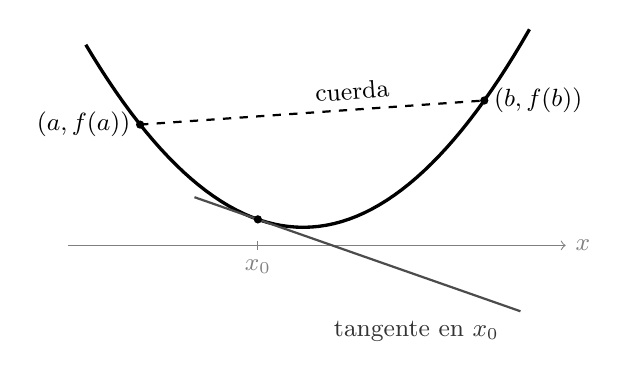
\begin{tikzpicture}[scale=1.15,font=\small,declare function={f(\x)=0.35*\x*\x+0.2;}]
  \draw[->,gray] (-2.6,0) -- (2.9,0) node[right] {$x$};
  \draw[very thick,domain=-2.4:2.5,samples=60] plot (\x,{f(\x)});
  \coordinate (A) at (-1.8,{f(-1.8)});
  \coordinate (B) at (2,{f(2)});
  \fill (A) circle (1.3pt) node[left] {$(a,f(a))$};
  \fill (B) circle (1.3pt) node[right] {$(b,f(b))$};
  \draw[thick,dashed] (A) -- (B) node[pos=0.62,above,sloped] {cuerda};
  \draw[thick,gray!60!black,domain=-1.2:2.4] plot (\x,{f(-0.5)+0.7*(-0.5)*(\x+0.5)});
  \fill (-0.5,{f(-0.5)}) circle (1.3pt);
  \node[gray!40!black] at (1.25,-0.95) {tangente en $x_0$};
  \draw[gray] (-0.5,0.05) -- (-0.5,-0.05) node[below] {$x_0$};
\end{tikzpicture}
\caption{Una función convexa queda por debajo de sus cuerdas (\cref{def:convexa}) y por encima de sus tangentes (\cref{teo:primer-orden}).}
\label{fig:convexa}
\end{figure}

\begin{lema}[Restricción a rectas]\label{lem:rectas}
Sea $C$ abierto y convexo. Una función $f\colon C\to\R$ es convexa si y solo si, para todo $x\in C$ y todo $v\in\R^{n}$, la función de una variable $\varphi(t)=f(x+tv)$ es convexa en el intervalo $\{t:x+tv\in C\}$.
\end{lema}

\begin{proof}
Si $f$ es convexa, para $t_1,t_2$ en el intervalo, $\varphi(\lambda t_1+(1-\lambda)t_2)=f\bigl(\lambda(x+t_1v)+(1-\lambda)(x+t_2v)\bigr)\le\lambda\varphi(t_1)+(1-\lambda)\varphi(t_2)$. Recíprocamente, dados $a,b\in C$, se toma $x=b$, $v=a-b$: entonces $\varphi(\lambda)=f(\lambda a+(1-\lambda)b)$ y la convexidad de $\varphi$ entre $t=0$ y $t=1$ es exactamente la desigualdad de la \cref{def:convexa}.
\end{proof}

\section{Condiciones de primer y segundo orden}

\begin{teorema}[Condición de primer orden]\label{teo:primer-orden}
Sea $C$ abierto y convexo y $f\colon C\to\R$ diferenciable. Entonces $f$ es convexa si y solo si
\[
f(b)\ge f(a)+\nabla f(a)\T(b-a)\qquad\text{para todo } a,b\in C.
\]
\end{teorema}

\begin{proof}
($\Rightarrow$) Para $\lambda\in(0,1]$, la convexidad da $f(a+\lambda(b-a))\le f(a)+\lambda\bigl(f(b)-f(a)\bigr)$, es decir,
\[
\frac{f(a+\lambda(b-a))-f(a)}{\lambda}\le f(b)-f(a).
\]
Cuando $\lambda\to 0^{+}$, el miembro izquierdo tiende a $\nabla f(a)\T(b-a)$ (\cref{prop:direccional}, sin normalizar la dirección), y se obtiene la desigualdad.

($\Leftarrow$) Sean $a,b\in C$, $\lambda\in[0,1]$ y $m=\lambda a+(1-\lambda)b$. Aplicando la hipótesis en el punto $m$ hacia $a$ y hacia $b$,
\[
f(a)\ge f(m)+\nabla f(m)\T(a-m),\qquad f(b)\ge f(m)+\nabla f(m)\T(b-m).
\]
Multiplicando por $\lambda$ y $1-\lambda$ y sumando, el término del gradiente se anula, porque $\lambda(a-m)+(1-\lambda)(b-m)=0$, y queda $\lambda f(a)+(1-\lambda)f(b)\ge f(m)$.
\end{proof}

La condición de primer orden dice que el plano tangente en cualquier punto es una cota inferior global de $f$: la información local del gradiente proporciona información global.

\begin{teorema}[Condición de segundo orden]\label{teo:segundo-orden}
Sea $C$ abierto y convexo y $f\in C^{2}(C)$. Entonces $f$ es convexa si y solo si $H_f(x)\succeq 0$ para todo $x\in C$. Si $H_f(x)\succ 0$ para todo $x\in C$, entonces $f$ es estrictamente convexa.
\end{teorema}

\begin{proof}
($\Leftarrow$) Sean $a,b\in C$. Por el \cref{teo:taylor}(i), $f(b)=f(a)+\nabla f(a)\T(b-a)+\tfrac12(b-a)\T H_f(\xi)(b-a)$ para un punto $\xi$ del segmento, que está en $C$. El último término es $\ge 0$, luego se cumple la condición de primer orden y $f$ es convexa por el \cref{teo:primer-orden}. Si $H_f\succ 0$ y $a\ne b$, el término es $>0$; repitiendo la demostración del \cref{teo:primer-orden} con desigualdades estrictas se obtiene la convexidad estricta.

($\Rightarrow$) Supóngase que existen $x\in C$ y $v$ con $v\T H_f(x)v<0$, y sea $\varphi(t)=f(x+tv)$. Por la demostración del \cref{teo:taylor}, $\varphi''(0)=v\T H_f(x)v<0$ y, por continuidad, $\varphi''<0$ en un intervalo alrededor de $0$. En ese intervalo $\varphi$ es estrictamente cóncava, luego no es convexa, y por el \cref{lem:rectas} tampoco lo es $f$.
\end{proof}

\begin{ejemplo}\label{ej:cuad-convexa}
$f(x,y)=x^{2}+xy+y^{2}$ tiene hessiano constante $\begin{pmatrix}2&1\\1&2\end{pmatrix}$, con autovalores~1 y~3. Por el \cref{teo:segundo-orden}, es estrictamente convexa en $\R^{2}$. En cambio, $x^{2}-y^{2}$, con autovalores $2$ y $-2$, no es convexa.
\end{ejemplo}

\begin{observacion}
El recíproco de la segunda parte del \cref{teo:segundo-orden} es falso: $f(x)=x^{4}$ es estrictamente convexa en $\R$, pero $f''(0)=0$.
\end{observacion}

\section{Mínimos de funciones convexas}

\begin{teorema}[Mínimos locales y globales]\label{teo:local-global}
Sea $f\colon C\to\R$ convexa. Todo mínimo local de $f$ es un mínimo global. Si además $f$ es diferenciable y $C$ es abierto, un punto $x^{*}$ es mínimo global si y solo si $\nabla f(x^{*})=0$.
\end{teorema}

\begin{proof}
Sea $x^{*}$ un mínimo local, con $f(x)\ge f(x^{*})$ si $\norm{x-x^{*}}<r$, y supóngase que existe $b\in C$ con $f(b)<f(x^{*})$. Para $\lambda\in(0,1)$ suficientemente pequeño, el punto $m=(1-\lambda)x^{*}+\lambda b$ está a distancia $\lambda\norm{b-x^{*}}<r$ de $x^{*}$, y por convexidad
\[
f(m)\le(1-\lambda)f(x^{*})+\lambda f(b)<f(x^{*}),
\]
lo que contradice que $x^{*}$ sea mínimo local. Para la segunda afirmación: si $x^{*}$ es mínimo, $\nabla f(x^{*})=0$ por el \cref{teo:fermat}; si $\nabla f(x^{*})=0$, el \cref{teo:primer-orden} da $f(b)\ge f(x^{*})$ para todo $b\in C$.
\end{proof}

Para funciones no convexas, $\nabla f=0$ solo es una condición necesaria. Para funciones convexas es también suficiente, y además global. Por eso el descenso de gradiente con una tasa adecuada resuelve los problemas convexos, como la regresión lineal y la regresión logística o softmax del módulo~8.

\section{Operaciones que conservan la convexidad}

\begin{proposicion}\label{prop:operaciones}
\begin{enumerate}
  \item Si $f_1,\dots,f_k$ son convexas y $w_1,\dots,w_k\ge 0$, entonces $\sum_i w_if_i$ es convexa.
  \item Si $f\colon\R^{m}\to\R$ es convexa, $A\in\R^{m\times n}$ y $b\in\R^{m}$, entonces $g(x)=f(Ax+b)$ es convexa.
  \item Si $f_1$ y $f_2$ son convexas, $\max(f_1,f_2)$ es convexa.
\end{enumerate}
\end{proposicion}

\begin{proof}
(i) Se multiplica la desigualdad de la \cref{def:convexa} de cada $f_i$ por $w_i\ge 0$ y se suma. (ii) Para $u,u'\in\R^{n}$, $A(\lambda u+(1-\lambda)u')+b=\lambda(Au+b)+(1-\lambda)(Au'+b)$, luego $g(\lambda u+(1-\lambda)u')=f\bigl(\lambda(Au+b)+(1-\lambda)(Au'+b)\bigr)\le\lambda g(u)+(1-\lambda)g(u')$. (iii) Para cada $i$, $f_i(\lambda a+(1-\lambda)b)\le\lambda f_i(a)+(1-\lambda)f_i(b)\le\lambda\max(f_1,f_2)(a)+(1-\lambda)\max(f_1,f_2)(b)$; basta tomar el máximo en $i$ del miembro izquierdo.
\end{proof}

\begin{proposicion}[Convexidad de log-suma-exp]\label{prop:lse-convexa}
La función $\LSE(z)=\ln\sum_{k=1}^{K}e^{z_k}$ es convexa en $\R^{K}$. Su hessiano es $H=\diag(p)-pp\T$ con $p=\softmax(z)$, y para todo $v\in\R^{K}$
\[
v\T Hv=\sum_i p_iv_i^{2}-\Bigl(\sum_i p_iv_i\Bigr)^{2}=\Var_{i\sim p}[v_i]\ge 0,
\]
con igualdad si y solo si $v$ es proporcional a $\uno$.
\end{proposicion}

\begin{proof}
El gradiente de $\LSE$ es $p=\softmax(z)$ (módulo~1, tema~4), y su jacobiano, por la \cref{prop:jac-softmax}, es $\diag(p)-pp\T$. Desarrollando la forma cuadrática se obtiene la varianza de la variable aleatoria que toma el valor $v_i$ con probabilidad $p_i$, que es no negativa. Como todas las $p_i$ son positivas, la varianza es nula si y solo si todos los $v_i$ son iguales. Se concluye por el \cref{teo:segundo-orden}.
\end{proof}

La demostración de~\cite[§3.1]{bv} obtiene la misma desigualdad mediante la de Cauchy--Schwarz.

\begin{corolario}[Convexidad de la entropía cruzada]\label{cor:ce-convexa}
La entropía cruzada $L(z)=-z_c+\LSE(z)$ es convexa en los logits $z$. Para un vector $x$ fijo, $W\mapsto -\ln\softmax(Wx)_c$ es convexa en $W$, y la pérdida media de la regresión softmax sobre un conjunto de datos es convexa en sus parámetros.
\end{corolario}

\begin{proof}
$L$ es la suma de una función afín y de $\LSE$, ambas convexas (\cref{prop:operaciones}(i) y \cref{prop:lse-convexa}). La aplicación $W\mapsto Wx$ es lineal, y la (ii) da la convexidad en $W$. La pérdida media es una suma con pesos positivos de funciones convexas.
\end{proof}

Para $z=(2,1,0)\T$, el hessiano de la entropía cruzada tiene autovalores $0$, $0{,}119$ y $0{,}371$. El autovalor nulo corresponde a la dirección $\uno$, a lo largo de la cual la pérdida es constante.

\section{Las redes profundas no son convexas}

\begin{proposicion}[Simetría y convexidad]\label{prop:simetria}
Sea $L\colon\R^{N}\to\R$ convexa. El conjunto de sus mínimos globales es convexo. En consecuencia, si $\theta_1$ y $\theta_2$ son mínimos globales y $\tfrac12(\theta_1+\theta_2)$ no lo es, $L$ no es convexa.
\end{proposicion}

\begin{proof}
Sea $m=\min L$ y $\theta_1,\theta_2$ con $L(\theta_1)=L(\theta_2)=m$. Para $\lambda\in[0,1]$, $L(\lambda\theta_1+(1-\lambda)\theta_2)\le\lambda m+(1-\lambda)m=m$, y como $m$ es el mínimo, se da la igualdad.
\end{proof}

En una red con una capa oculta, intercambiar dos neuronas ocultas (junto con sus pesos de entrada y de salida) no cambia la función calculada. Si $\theta_1$ es un mínimo, la permutación $\theta_2$ también lo es, pero el punto medio promedia las dos neuronas y, en general, calcula otra función con pérdida mayor. Por la \cref{prop:simetria}, la pérdida no es convexa.

\begin{ejemplo}[Una red lineal de dos capas]\label{ej:red-lineal}
La red más sencilla con dos capas calcula $\hat y=w_2w_1x$. Con un único dato $(x,y)=(1,1)$ y pérdida cuadrática, $L(w_1,w_2)=(1-w_1w_2)^{2}$. Los mínimos globales ($L=0$) forman la hipérbola $w_1w_2=1$, que no es un conjunto convexo: $(1,1)$ y $(-1,-1)$ son mínimos, pero su punto medio $(0,0)$ da $L=1$. Además,
\[
H_L(w_1,w_2)=\begin{pmatrix}2w_2^{2}&4w_1w_2-2\\4w_1w_2-2&2w_1^{2}\end{pmatrix},\qquad H_L(0,0)=\begin{pmatrix}0&-2\\-2&0\end{pmatrix},
\]
con autovalores $\pm 2$: el origen es un punto de silla. La función calculada, $w_1w_2x$, es lineal en $x$; la falta de convexidad procede solo de la composición de dos capas.
\end{ejemplo}

\begin{figure}[h]
\centering
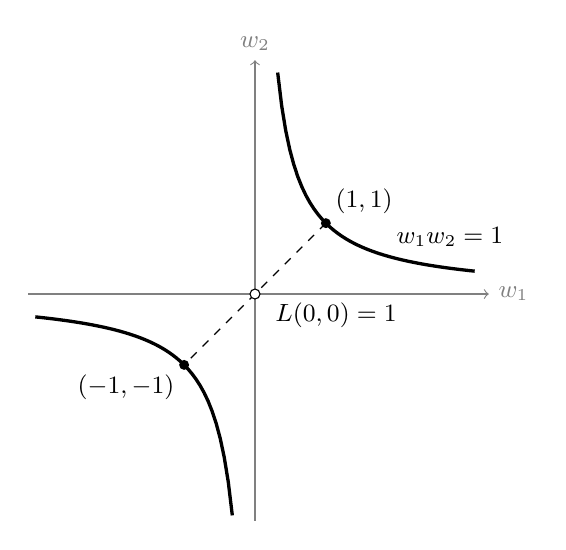
\begin{tikzpicture}[scale=0.9,font=\small]
  \draw[->,gray] (-3.2,0) -- (3.3,0) node[right] {$w_1$};
  \draw[->,gray] (0,-3.2) -- (0,3.3) node[above] {$w_2$};
  \draw[very thick,domain=0.32:3.1,samples=50] plot (\x,{1/\x});
  \draw[very thick,domain=-3.1:-0.32,samples=50] plot (\x,{1/\x});
  \fill (1,1) circle (2pt) node[above right] {$(1,1)$};
  \fill (-1,-1) circle (2pt) node[below left] {$(-1,-1)$};
  \draw[dashed] (1,1) -- (-1,-1);
  \draw[fill=white] (0,0) circle (2pt);
  \node[right] at (0.15,-0.3) {$L(0,0)=1$};
  \node at (2.75,0.8) {$w_1w_2=1$};
\end{tikzpicture}
\caption{Mínimos globales de $L(w_1,w_2)=(1-w_1w_2)^{2}$ (\cref{ej:red-lineal}). El segmento que une dos mínimos sale del conjunto de mínimos: la pérdida no es convexa.}
\label{fig:hiperbola}
\end{figure}

\begin{observacion}[Conexión con los LLM]
La pérdida de un Transformer como función de sus pesos no es convexa, y no hay garantía teórica general de que el descenso de gradiente alcance un mínimo global. En la práctica, el entrenamiento funciona de manera muy robusta gracias a la sobreparametrización, la inicialización cuidadosa, la normalización y los métodos adaptativos (módulos~7 y~11). La explicación teórica completa de este hecho sigue siendo un problema abierto.
\end{observacion}

\begin{lecturas}
\item Boyd y Vandenberghe~\cite{bv}, §3.1 «Basic properties and examples» (definición, condiciones de primer y segundo orden, ejemplos, incluida log-suma-exp), §3.2 «Operations that preserve convexity» y §4.2 «Convex optimization» (óptimos locales y globales).
\item Stanford EE364a~\cite{ee364a}, transparencias «Convex functions».
\item Goodfellow, Bengio y Courville~\cite{gbc}, §4.3 (optimización convexa frente a no convexa).
\end{lecturas}

\section*{Ejercicios del tema 5}
\addcontentsline{toc}{section}{Ejercicios del tema 5}

\begin{ejercicio}{1}{eje:5-vf}
Justifique si son verdaderas o falsas: (a) toda función $C^{2}$ con hessiano semidefinido positivo en todo $\R^{n}$ es convexa; (b) el producto de dos funciones convexas es convexo; (c) el máximo de dos funciones convexas es convexo.
\end{ejercicio}

\begin{ejercicio}{2}{eje:5-hessianos}
Decida, con el \cref{teo:segundo-orden}, cuáles de las siguientes funciones de $\R^{2}$ son convexas y cuáles estrictamente convexas: (a) $x^{2}+xy+y^{2}$; (b) $x^{2}-4xy+y^{2}$; (c) $e^{x+y}$; (d) $x^{4}+y^{2}$.
\end{ejercicio}

\begin{ejercicio}{2}{eje:5-boyd}
En el dominio $\R^{2}_{++}=\{(x_1,x_2):x_1>0,\ x_2>0\}$, determine si cada función es convexa, cóncava o ninguna de las dos: (a) $f(x)=x_1x_2$; (b) $f(x)=1/(x_1x_2)$; (c) $f(x)=x_1^{2}/x_2$.
\fuente{adaptado de Boyd y Vandenberghe~\cite{bv}, ejercicio~3.16 (selección de casos; se omite el estudio de la cuasiconvexidad).}
\end{ejercicio}

\begin{ejercicio}{2}{eje:5-red}
Sea $L(w_1,w_2)=(2-w_1w_2)^{2}$, la pérdida de una red lineal de dos capas con el dato $(x,y)=(1,2)$. (a) Compruebe que $(1,2)$ y $(2,1)$ son mínimos globales y evalúe $L$ en su punto medio. (b) Calcule $H_L(0,0)$ y clasifique el origen. (c) Concluya sobre la convexidad de $L$.
\end{ejercicio}

\begin{ejercicio}{3}{eje:5-softmax-W}
Demuestre directamente, a partir de la \cref{def:convexa} y de la convexidad de $\varphi(z)=-z_c+\LSE(z)$, que $L(W)=\varphi(Wx)$ es convexa en $W$ para $x$ fijo. Explique qué paso de la demostración falla para una red $\varphi(W_2\,\sigma(W_1x))$ con una función de activación no lineal $\sigma$.
\end{ejercicio}

\begin{ejercicio}{3}{eje:5-unico}
Sea $f\colon C\to\R$ estrictamente convexa. Demuestre que $f$ tiene a lo sumo un mínimo global. Demuestre que la entropía cruzada $L(z)$ no es estrictamente convexa en $\R^{K}$. Demuestre que $L_\mu(z)=L(z)+\tfrac{\mu}{2}\norm{z}^{2}$, con $\mu>0$, es estrictamente convexa, que tiene a lo sumo un mínimo y que, si lo tiene, sus componentes suman cero.
\end{ejercicio}

% =====================================================================
\chapter{Diferenciación numérica y comprobación de gradientes}
\label{tema:6}
% =====================================================================

Un error en la implementación de un gradiente no suele provocar un fallo visible: el entrenamiento avanza, pero peor de lo que debería. La herramienta estándar para detectarlo es comparar el gradiente analítico con una aproximación por diferencias finitas. Este tema analiza el error de truncamiento de las diferencias finitas con el teorema de Taylor, el error de redondeo de la aritmética de coma flotante y el compromiso entre ambos, y describe el procedimiento de comprobación de gradientes. Se sigue~\cite[§4.1]{gbc} y las notas de~\cite{cs231n}.

\section{Diferencias finitas}

\begin{definicion}[Diferencias finitas]\label{def:diferencias}
Sea $f\colon\R^{n}\to\R$ y $h>0$. Las \emph{diferencias hacia delante} y \emph{centrada} en la coordenada $i$ son
\[
\Delta_i^{+}f(x)=\frac{f(x+h\,e_i)-f(x)}{h},\qquad
\Delta_i^{c}f(x)=\frac{f(x+h\,e_i)-f(x-h\,e_i)}{2h}.
\]
Ambas aproximan $\partial f/\partial x_i(x)$ cuando $h\to 0$.
\end{definicion}

\begin{proposicion}[Error de truncamiento]\label{prop:truncamiento}
Sea $\phi\colon\R\to\R$ y $x\in\R$.
\begin{enumerate}
  \item Si $\phi\in C^{2}$, existe $\xi\in(x,x+h)$ tal que $\dfrac{\phi(x+h)-\phi(x)}{h}=\phi'(x)+\dfrac{h}{2}\,\phi''(\xi)$.
  \item Si $\phi\in C^{3}$, existe $\xi\in(x-h,x+h)$ tal que $\dfrac{\phi(x+h)-\phi(x-h)}{2h}=\phi'(x)+\dfrac{h^{2}}{6}\,\phi'''(\xi)$.
\end{enumerate}
En consecuencia, el error de la diferencia hacia delante es $O(h)$ y el de la centrada es $O(h^{2})$.
\end{proposicion}

\begin{proof}
(i) Es el teorema de Taylor con resto de Lagrange de orden~2: $\phi(x+h)=\phi(x)+h\phi'(x)+\tfrac{h^{2}}{2}\phi''(\xi)$; basta restar $\phi(x)$ y dividir por $h$.

(ii) Con resto de orden~3, $\phi(x\pm h)=\phi(x)\pm h\phi'(x)+\tfrac{h^{2}}{2}\phi''(x)\pm\tfrac{h^{3}}{6}\phi'''(\xi_\pm)$, con $\xi_+\in(x,x+h)$ y $\xi_-\in(x-h,x)$. Al restar, los términos de orden par se cancelan:
\[
\frac{\phi(x+h)-\phi(x-h)}{2h}=\phi'(x)+\frac{h^{2}}{6}\cdot\frac{\phi'''(\xi_+)+\phi'''(\xi_-)}{2}.
\]
La media de los dos valores de $\phi'''$ está entre ambos y, por el teorema de los valores intermedios aplicado a la función continua $\phi'''$, es igual a $\phi'''(\xi)$ para algún $\xi\in(x-h,x+h)$.
\end{proof}

Para una función de varias variables se aplica la proposición a $\phi(t)=f(x+t\,e_i)$.

\begin{ejemplo}\label{ej:exp}
Para $f(x)=e^{x}$ en $x=0$, con derivada exacta~1, la \cref{prop:truncamiento} predice errores de $h/2$ y $h^{2}/6$ aproximadamente. El \cref{tab:exp} lo confirma: al dividir $h$ entre~10, el error hacia delante se divide entre~10 y el centrado entre~100.
\end{ejemplo}

\begin{table}[h]
\centering\small
\caption{Diferencias finitas para $f(x)=e^{x}$ en $x=0$ (\cref{ej:exp}).}\label{tab:exp}
\begin{tabular}{@{}lllll@{}}
\toprule
$h$ & Hacia delante & Error & Centrada & Error \\
\midrule
$0{,}1$ & $1{,}051709$ & $5{,}17\cdot 10^{-2}$ & $1{,}001668$ & $1{,}67\cdot 10^{-3}$ \\
$0{,}01$ & $1{,}005017$ & $5{,}02\cdot 10^{-3}$ & $1{,}0000167$ & $1{,}67\cdot 10^{-5}$ \\
$0{,}001$ & $1{,}000500$ & $5{,}00\cdot 10^{-4}$ & $1{,}00000017$ & $1{,}67\cdot 10^{-7}$ \\
\bottomrule
\end{tabular}
\end{table}

\section{Error de redondeo y elección del paso}

En aritmética de coma flotante, cada evaluación de $f$ tiene un error relativo de redondeo del orden del \emph{épsilon de la máquina} $\varepsilon_{\text{máq}}$: unos $1{,}1\cdot 10^{-16}$ en doble precisión (fp64), $6{,}0\cdot 10^{-8}$ en simple precisión (fp32) y $3{,}9\cdot 10^{-3}$ en el formato bf16 que se usa para entrenar modelos de lenguaje~\cite[§4.1]{gbc}. Al restar dos valores casi iguales, $f(x+h)$ y $f(x-h)$, los errores absolutos, de tamaño $\varepsilon_{\text{máq}}\abs{f(x)}$, no disminuyen, y al dividir por $2h$ se amplifican.

\begin{proposicion}[Paso óptimo de la diferencia centrada]\label{prop:h-optimo}
Supóngase que cada evaluación de $f$ tiene un error absoluto a lo sumo $\varepsilon\abs{f}$ y que $\abs{\phi'''}\le M$ cerca de $x$. Entonces el error total de la diferencia centrada está acotado por
\[
E(h)=\frac{\varepsilon\abs{f}}{h}+\frac{M h^{2}}{6},
\]
que alcanza su mínimo en
\[
h^{*}=\Bigl(\frac{3\varepsilon\abs{f}}{M}\Bigr)^{1/3},\qquad E(h^{*})=\frac{M}{2}\,(h^{*})^{2}=O\bigl(\varepsilon^{2/3}\bigr).
\]
\end{proposicion}

\begin{proof}
El numerador calculado difiere del exacto en a lo sumo $2\varepsilon\abs{f}$, y al dividir por $2h$ se obtiene el primer término; el segundo es la cota de truncamiento de la \cref{prop:truncamiento}(ii). En $(0,\infty)$, $E'(h)=-\varepsilon\abs{f}/h^{2}+Mh/3$ se anula solo en $h^{*}$, con $E'<0$ antes y $E'>0$ después, luego $h^{*}$ es el mínimo. Sustituyendo $\varepsilon\abs{f}=M(h^{*})^{3}/3$ se obtiene $E(h^{*})=M(h^{*})^{2}/3+M(h^{*})^{2}/6=M(h^{*})^{2}/2$.
\end{proof}

Con $\abs{f}\approx M\approx 1$ y doble precisión, $h^{*}\approx(3{,}3\cdot 10^{-16})^{1/3}\approx 7\cdot 10^{-6}$ y el error mínimo es del orden de $10^{-11}$. Pasos más pequeños empeoran el resultado (\cref{fig:error-h}). En simple precisión, $h^{*}\approx 6\cdot 10^{-3}$ y el error mínimo es del orden de $10^{-5}$; en bf16 la comprobación carece de sentido. Por ello, los gradientes se comprueban siempre en doble precisión.

\begin{figure}[h]
\centering
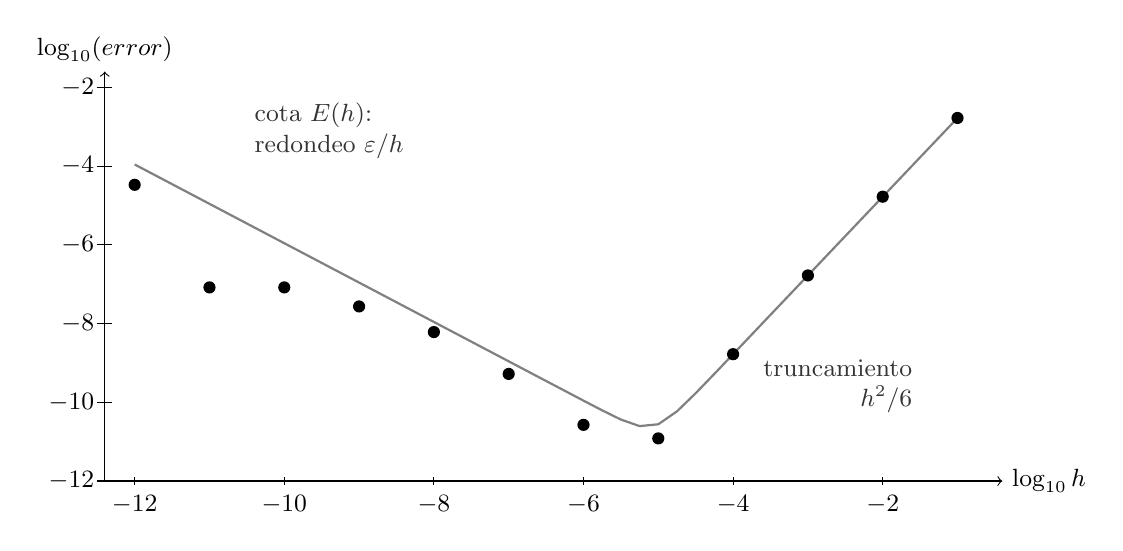
\begin{tikzpicture}[x=0.95cm,y=0.5cm,font=\small]
  \draw[->] (-12.4,-12) -- (-0.4,-12) node[right] {$\log_{10}h$};
  \draw[->] (-12.4,-12) -- (-12.4,-1.6) node[above] {$\log_{10}(\text{error})$};
  \foreach \t in {-12,-10,-8,-6,-4,-2} {\draw (\t,-12.1) -- (\t,-11.9) node[below=3pt] {$\t$};}
  \foreach \e in {-12,-10,-8,-6,-4,-2} {\draw (-12.5,\e) -- (-12.3,\e) node[left=3pt] {$\e$};}
  \draw[thick,gray] plot coordinates {(-12.00,-3.959) (-11.75,-4.209) (-11.50,-4.459) (-11.25,-4.709) (-11.00,-4.959) (-10.75,-5.209) (-10.50,-5.459) (-10.25,-5.709) (-10.00,-5.959) (-9.75,-6.209) (-9.50,-6.459) (-9.25,-6.709) (-9.00,-6.959) (-8.75,-7.209) (-8.50,-7.459) (-8.25,-7.709) (-8.00,-7.959) (-7.75,-8.209) (-7.50,-8.459) (-7.25,-8.709) (-7.00,-8.959) (-6.75,-9.209) (-6.50,-9.459) (-6.25,-9.708) (-6.00,-9.958) (-5.75,-10.205) (-5.50,-10.438) (-5.25,-10.605) (-5.00,-10.558) (-4.75,-10.230) (-4.50,-9.769) (-4.25,-9.277) (-4.00,-8.778) (-3.75,-8.278) (-3.50,-7.778) (-3.25,-7.278) (-3.00,-6.778) (-2.75,-6.278) (-2.50,-5.778) (-2.25,-5.278) (-2.00,-4.778) (-1.75,-4.278) (-1.50,-3.778) (-1.25,-3.278) (-1.00,-2.778)};
  \foreach \p in {(-1,-2.778),(-2,-4.778),(-3,-6.778),(-4,-8.778),(-5,-10.917),(-6,-10.573),(-7,-9.279),(-8,-8.216),(-9,-7.565),(-10,-7.082),(-11,-7.082),(-12,-4.476)} {\fill \p circle (2.2pt);}
  \node[gray!40!black,align=left] at (-9.4,-3.1) {cota $E(h)$:\\ redondeo $\varepsilon/h$};
  \node[gray!40!black,align=right] at (-2.6,-9.6) {truncamiento\\ $h^{2}/6$};
\end{tikzpicture}
\caption{Error de la diferencia centrada para $f(x)=e^{x}$ en $x=0$, calculada en doble precisión (puntos), y cota $E(h)$ de la \cref{prop:h-optimo} con $\varepsilon=1{,}1\cdot 10^{-16}$ y $\abs{f}=M=1$ (línea). A la derecha domina el truncamiento (pendiente~2); a la izquierda, el redondeo (pendiente~$-1$). El error medido mínimo, $1{,}2\cdot 10^{-11}$, se obtiene con $h=10^{-5}$.}
\label{fig:error-h}
\end{figure}

\section{Comprobación de gradientes}

\begin{definicion}[Error relativo]\label{def:error-relativo}
Sean $a$ una componente del gradiente analítico y $n$ la correspondiente aproximación numérica, no ambas nulas. Su \emph{error relativo} es
\[
r(a,n)=\frac{\abs{a-n}}{\max(\abs{a},\abs{n})}.
\]
\end{definicion}

El error relativo, a diferencia del absoluto, no depende de la escala del gradiente. Las notas de~\cite{cs231n} proponen como orientación, para comprobaciones en doble precisión: $r>10^{-2}$ indica casi con seguridad un error; $10^{-4}<r<10^{-2}$ es sospechoso, salvo en funciones con puntos no derivables; $r\le 10^{-7}$ indica un gradiente correcto. En redes profundas, el error relativo tiende a crecer con la profundidad.

\begin{proposicion}[Coste de la comprobación]\label{prop:coste-fd}
Calcular el gradiente completo de $f\colon\R^{N}\to\R$ por diferencias centradas requiere $2N$ evaluaciones de $f$. En cambio, para una dirección $v\in\R^{N}$, la derivada direccional $\nabla f(x)\T v$ se aproxima con dos evaluaciones:
\[
\nabla f(x)\T v=\frac{f(x+hv)-f(x-hv)}{2h}+O(h^{2}).
\]
\end{proposicion}

\begin{proof}
La primera afirmación se sigue de la \cref{def:diferencias}: dos evaluaciones por coordenada. Para la segunda, se aplica la \cref{prop:truncamiento}(ii) a $\phi(t)=f(x+tv)$, cuya derivada en $0$ es $\nabla f(x)\T v$ por el \cref{lem:curva}.
\end{proof}

La retropropagación obtiene el gradiente completo con un coste equivalente a unas pocas evaluaciones de $f$ (\cref{prop:modos}). Las diferencias finitas, por tanto, no sirven para entrenar, sino para \emph{verificar}. El procedimiento habitual es el siguiente~\cite{cs231n}:
\begin{enumerate}[label=\arabic*.]
  \item usar doble precisión y un modelo o un lote pequeños, con pocos datos;
  \item comparar componentes elegidas al azar, o derivadas direccionales en direcciones aleatorias, mediante el error relativo;
  \item tomar $h$ del orden de $10^{-5}$ y repetir con $10^{-4}$ y $10^{-6}$ si el resultado es dudoso;
  \item vigilar los puntos no derivables, como $t=0$ en ReLU: si $x-h$ y $x+h$ quedan a distintos lados de uno de ellos, la aproximación numérica no es fiable.
\end{enumerate}

\begin{observacion}[Conexión con los LLM]
Las bibliotecas de diferenciación automática incluyen utilidades de comprobación de este tipo, como \texttt{torch.autograd.gradcheck} en PyTorch, que comparan los gradientes analítico y numérico en doble precisión. Se usan al implementar una operación nueva, por ejemplo una variante de la atención, antes de emplearla en un modelo grande.
\end{observacion}

\begin{lecturas}
\item Goodfellow, Bengio y Courville~\cite{gbc}, §4.1 «Overflow and Underflow».
\item Stanford CS231n~\cite{cs231n}, notas «Neural Networks Part 3», sección «Gradient checks».
\item Deisenroth, Faisal y Ong~\cite{mml}, §5.1 (Taylor en una variable).
\end{lecturas}

\section*{Ejercicios del tema 6}
\addcontentsline{toc}{section}{Ejercicios del tema 6}

\begin{ejercicio}{1}{eje:6-porque}
¿Por qué no se entrena un LLM calculando el gradiente por diferencias finitas, si son tan sencillas de implementar? ¿Para qué se usan entonces?
\end{ejercicio}

\begin{ejercicio}{2}{eje:6-cubo}
Para $f(x)=x^{3}$ en $x=1$, calcule la diferencia hacia delante y la centrada con $h=0{,}1$ y $h=0{,}01$. ¿Cómo disminuye cada error al dividir $h$ entre~10? Compare con la \cref{prop:truncamiento}.
\end{ejercicio}

\begin{ejercicio}{2}{eje:6-direccional}
Sea $f(x,y)=x^{2}y+3y$. Compruebe el gradiente $\nabla f(2,1)=(4,7)\T$ en la dirección $v=(1,1)\T$ mediante la \cref{prop:coste-fd} con $h=0{,}01$, y calcule el error relativo.
\end{ejercicio}

\begin{ejercicio}{2}{eje:6-cs231n}
Una comprobación de gradientes en doble precisión da los siguientes pares (analítico, numérico): (a) $(1;\,1{,}0000001)$; (b) $(0{,}5;\,0{,}52)$; (c) $(10^{-3};\,1{,}0005\cdot 10^{-3})$. Calcule el error relativo de cada par y valore el resultado. (d) Para $f(x)=\max(0,x)$ en $x=10^{-6}$ con $h=10^{-5}$, calcule la diferencia centrada y su error relativo respecto de la derivada exacta, y explique el resultado.
\fuente{adaptado de Stanford CS231n~\cite{cs231n}, notas «Neural Networks Part 3», sección «Gradient checks» (criterios de error relativo y puntos no derivables).}
\end{ejercicio}

\begin{ejercicio}{2}{eje:6-fermi}
Se desea comprobar por diferencias centradas el gradiente completo de un modelo de $7\cdot 10^{9}$ parámetros. ¿Cuántas evaluaciones de la pérdida se necesitan? Si cada una tarda 1~s, ¿cuántos años se tardaría? ¿Qué se haría en su lugar?
\end{ejercicio}

\begin{ejercicio}{3}{eje:6-hoptimo}
Demuestre la \cref{prop:h-optimo} con todo detalle. Calcule $h^{*}$ y $E(h^{*})$ para $f(x)=e^{x}$ en $x=0$ con $\varepsilon=1{,}1\cdot 10^{-16}$ y compárelos con la \cref{fig:error-h}. Repita el razonamiento para la diferencia hacia delante y demuestre que, en ese caso, el paso óptimo es de orden $\varepsilon^{1/2}$ y el error mínimo también.
\end{ejercicio}


\appendix
% =====================================================================
\chapter{Soluciones de los ejercicios}
\label{ap:soluciones}
% =====================================================================

Cada solución se presenta en cinco partes: datos, planteamiento, desarrollo, resultado y comprobación. En los pasos intermedios se redondea a cuatro cifras significativas salvo que se indique otra cosa; los resultados exactos se dan como fracción o con radicales cuando existen.

% ---------------------------------------------------------------------
\section{Tema 1}

\begin{solucion}{eje:1-vf}
\planteamiento contrastar cada afirmación con los resultados del \cref{tema:1}.
\pasos
\begin{enumerate}[label=(\alph*)]
  \item \textbf{Verdadera} si $f$ es diferenciable. Si $r(t)$ recorre una curva de nivel, $f(r(t))=c$ y el \cref{cor:nivel} da $\nabla f(r(t))\T r'(t)=0$: el gradiente es ortogonal a la tangente.
  \item \textbf{Verdadera.} Por el \cref{teo:max-ascenso}, $D_uf\ge-\norm{\nabla f}$, con igualdad solo en $u=-\nabla f/\norm{\nabla f}$.
  \item \textbf{Falsa.} La función $f(x,y)=xy/(x^{2}+y^{2})$, con $f(0,0)=0$, tiene ambas parciales nulas en el origen, pero $f(t,t)=1/2$ para $t\ne 0$; no es continua en $(0,0)$ y, por tanto, no es diferenciable allí.
\end{enumerate}
\resultado \textbf{(a) verdadera; (b) verdadera; (c) falsa.}
\comprobacion en (c), si $f$ fuera diferenciable en el origen, su gradiente sería $(0,0)\T$ (\cref{prop:grad-parciales}) y se tendría $f(t,t)=o(\abs{t})\to 0$, en contradicción con $f(t,t)=1/2$.
\end{solucion}

\begin{solucion}{eje:1-gradiente}
\datos $f(x,y)=x^{3}+2xy^{2}$; punto $(1,2)$; $u=(1,1)\T/\sqrt2$.
\planteamiento derivar respecto de cada variable con la otra fija y aplicar la \cref{prop:direccional}.
\pasos
\begin{enumerate}[label=\arabic*.]
  \item $\partial f/\partial x=3x^{2}+2y^{2}$; en $(1,2)$: $3+8=11$.
  \item $\partial f/\partial y=4xy$; en $(1,2)$: $8$.
  \item $\nabla f(1,2)=(11,8)\T$ y $\norm{\nabla f(1,2)}=\sqrt{121+64}=\sqrt{185}\approx 13{,}60$.
  \item $D_uf(1,2)=(11+8)/\sqrt2=19/\sqrt2\approx 13{,}44$.
\end{enumerate}
\resultado \textbf{$\nabla f(1,2)=(11,8)\T$; $\norm{\nabla f}=\sqrt{185}\approx 13{,}60$; $D_uf=19/\sqrt2\approx 13{,}44$.}
\comprobacion $13{,}44<13{,}60$, como exige el \cref{teo:max-ascenso}. Las dos cifras son próximas porque el ángulo entre $u$ y $\nabla f$ es pequeño: su coseno es $13{,}44/13{,}60\approx 0{,}988$.
\end{solucion}

\begin{solucion}{eje:1-d2l}
\datos $f(x)=3x_1^{2}+5e^{x_2}$; punto $(1,0)$; dirección $(3,4)\T$.
\planteamiento calcular el gradiente, normalizar la dirección y usar $D_uf=\nabla f\T u$.
\pasos
\begin{enumerate}[label=\arabic*.]
  \item $\nabla f(x)=(6x_1,\;5e^{x_2})\T$.
  \item En $(1,0)$: $\nabla f=(6,\;5e^{0})\T=(6,5)\T$.
  \item $\norm{(3,4)}=5$, luego $u=(0{,}6;\,0{,}8)\T$.
  \item $D_uf(1,0)=6\cdot 0{,}6+5\cdot 0{,}8=3{,}6+4=7{,}6$.
  \item $\norm{\nabla f(1,0)}=\sqrt{36+25}=\sqrt{61}\approx 7{,}810$.
\end{enumerate}
\resultado \textbf{$\nabla f(1,0)=(6,5)\T$; $D_uf=7{,}6\le\sqrt{61}\approx 7{,}810$.}
\comprobacion la diferencia centrada en $x_2$ con $h=0{,}01$ da $5\,(e^{0{,}01}-e^{-0{,}01})/0{,}02=5\cdot 1{,}0000167\approx 5{,}0001$.
\end{solucion}

\begin{solucion}{eje:1-norma}
\datos $f(x)=\norm{x}=\bigl(\sum_ix_i^{2}\bigr)^{1/2}$; $x=(3,4)\T$.
\planteamiento regla de la cadena en una variable con $s=\sum_ix_i^{2}$ y $f=s^{1/2}$.
\pasos
\begin{enumerate}[label=\arabic*.]
  \item $\partial s/\partial x_i=2x_i$ y $d(s^{1/2})/ds=\tfrac12 s^{-1/2}$.
  \item $\partial f/\partial x_i=\tfrac12 s^{-1/2}\cdot 2x_i=x_i/\norm{x}$, luego $\nabla f(x)=x/\norm{x}$, el vector unitario en la dirección de $x$. Las parciales son continuas fuera del origen, luego $f$ es diferenciable allí (\cref{teo:C1}).
  \item En $(3,4)$: $\norm{x}=5$ y $\nabla f=(0{,}6;\,0{,}8)\T$.
  \item En $x=0$: $f(t\,e_1)=\abs{t}$, cuyo cociente $\abs{t}/t$ vale $-1$ para $t<0$ y $+1$ para $t>0$. La parcial $\partial f/\partial x_1(0)$ no existe y $f$ no es diferenciable en el origen.
  \item El recorte por norma sustituye $g$ por $c\,g/\norm{g}$ cuando $\norm{g}>c$: conserva la dirección $\nabla\norm{g}=g/\norm{g}$ y fija la longitud en $c$.
\end{enumerate}
\resultado \textbf{$\nabla\norm{x}=x/\norm{x}$ para $x\ne 0$; en $(3,4)$ vale $(0{,}6;\,0{,}8)\T$; en $x=0$ no existe.}
\comprobacion $\norm{\nabla f(x)}=1$ para todo $x\ne 0$: alejarse radialmente del origen aumenta la norma a razón de una unidad por unidad recorrida.
\end{solucion}

\begin{solucion}{eje:1-mit}
\datos $f(x,y)=x^{3}-3x^{2}+xy-y^{2}+x+y$; punto $(1,1/2)$.
\planteamiento por el \cref{teo:max-ascenso}, el máximo se alcanza en $\nabla f/\norm{\nabla f}$, el mínimo en la dirección opuesta, y la derivada direccional es nula en las direcciones ortogonales al gradiente.
\pasos
\begin{enumerate}[label=\arabic*.]
  \item $f_x=3x^{2}-6x+y+1$; en $(1,1/2)$: $3-6+0{,}5+1=-1{,}5$.
  \item $f_y=x-2y+1$; en $(1,1/2)$: $1-1+1=1$.
  \item $\nabla f=(-3/2,\,1)\T$ y $\norm{\nabla f}=\sqrt{9/4+1}=\sqrt{13}/2\approx 1{,}803$.
  \item Máximo: $u=(-3,2)\T/\sqrt{13}\approx(-0{,}8321;\,0{,}5547)$, con $D_uf=\sqrt{13}/2\approx 1{,}803$.
  \item Mínimo: $u=(3,-2)\T/\sqrt{13}$, con $D_uf\approx-1{,}803$.
  \item Nulas: los vectores unitarios ortogonales a $(-3,2)$, es decir,
  \[u=\pm(2,3)\T/\sqrt{13}\approx\pm(0{,}5547;\,0{,}8321).\]
\end{enumerate}
\resultado \textbf{máximo $\sqrt{13}/2\approx 1{,}803$ en $(-3,2)\T/\sqrt{13}$; mínimo $-1{,}803$ en $(3,-2)\T/\sqrt{13}$; nula en $\pm(2,3)\T/\sqrt{13}$.}
\comprobacion $(-3,2)\cdot(2,3)=-6+6=0$, y $\nabla f\T(-3,2)\T/\sqrt{13}=(4{,}5+2)/\sqrt{13}=6{,}5/3{,}606\approx 1{,}803$.
\end{solucion}

\begin{solucion}{eje:1-minimo}
\datos $g=\nabla f(x)\ne 0$; $u$ unitario; $f(x,y)=x^{2}+y^{2}$ y $r(t)=\sqrt c\,(\cos t,\sin t)\T$.
\planteamiento Cauchy--Schwarz para la cota y el \cref{lem:curva} para la ortogonalidad.
\pasos
\begin{enumerate}[label=\arabic*.]
  \item Por la \cref{prop:direccional}, $D_uf(x)=g\T u$.
  \item Por Cauchy--Schwarz, $\abs{g\T u}\le\norm{g}\,\norm{u}=\norm{g}$; en particular, $g\T u\ge-\norm{g}$.
  \item La cota se alcanza: para $u^{-}=-g/\norm{g}$, que es unitario porque $g\ne 0$, se tiene $g\T u^{-}=-\norm{g}^{2}/\norm{g}=-\norm{g}$.
  \item Unicidad: la igualdad en Cauchy--Schwarz exige $u=\alpha g$; con $\norm u=1$, $\alpha=\pm1/\norm{g}$, y solo el signo negativo da $-\norm g$.
  \item Circunferencias: $f(r(t))=c(\cos^{2}t+\sin^{2}t)=c$ para todo $t$, y $r'(t)=\sqrt c\,(-\sin t,\cos t)\T$.
  \item $\nabla f(r(t))=2r(t)=2\sqrt c\,(\cos t,\sin t)\T$, luego $\nabla f(r(t))\T r'(t)=2c(-\cos t\sin t+\sin t\cos t)=0$.
\end{enumerate}
\resultado \textbf{$\min_{\norm u=1}D_uf(x)=-\norm{\nabla f(x)}$, alcanzado solo en $u=-\nabla f/\norm{\nabla f}$; en las circunferencias, el gradiente es radial y ortogonal a la tangente.} $\blacksquare$
\comprobacion la derivada de la constante $f(r(t))=c$ es nula, como debe ser por el \cref{cor:nivel}.
\end{solucion}

% ---------------------------------------------------------------------
\section{Tema 2}

\begin{solucion}{eje:2-formas}
\datos $g\colon\R^{5}\to\R^{3}$, $h\colon\R^{3}\to\R^{2}$, $f\colon\R^{2}\to\R$.
\planteamiento el jacobiano de una función $\R^{n}\to\R^{m}$ es $m\times n$ (\cref{def:jacobiano}).
\pasos
\begin{enumerate}[label=\arabic*.]
  \item $J_g$ es $3\times 5$, $J_h$ es $2\times 3$ y $J_f$ es $1\times 2$.
  \item Por el \cref{teo:cadena}, $J_{f\circ h\circ g}=J_f\,J_h\,J_g$: $(1\times 2)(2\times 3)(3\times 5)=1\times 5$.
  \item El gradiente es la traspuesta: un vector de $\R^{5}$, de forma $5\times 1$.
\end{enumerate}
\resultado \textbf{$3\times 5$, $2\times 3$, $1\times 2$; la composición tiene jacobiano $1\times 5$ y gradiente en $\R^{5}$.}
\comprobacion en cada producto coinciden las dimensiones interiores ($2$ y $3$), y el gradiente tiene la forma de la variable de entrada.
\end{solucion}

\begin{solucion}{eje:2-producto}
\datos $F=uv$ con $u=x+y^{2}$, $v=x^{2}-y$; punto $(1,2)$.
\planteamiento \cref{cor:cadena-escalar}: $\partial F/\partial x=F_u\,u_x+F_v\,v_x$ y análogamente para $y$.
\pasos
\begin{enumerate}[label=\arabic*.]
  \item Valores: $u=1+4=5$ y $v=1-2=-1$.
  \item Derivadas exteriores: $F_u=v=-1$ y $F_v=u=5$.
  \item Derivadas interiores: $u_x=1$, $u_y=2y=4$, $v_x=2x=2$, $v_y=-1$.
  \item $\partial F/\partial x=(-1)\cdot 1+5\cdot 2=9$.
  \item $\partial F/\partial y=(-1)\cdot 4+5\cdot(-1)=-9$.
\end{enumerate}
\resultado \textbf{$\partial F/\partial x=9$ y $\partial F/\partial y=-9$ en $(1,2)$.}
\comprobacion $F=x^{3}-xy+x^{2}y^{2}-y^{3}$, luego $F_x=3x^{2}-y+2xy^{2}=3-2+8=9$ y $F_y=-x+2x^{2}y-3y^{2}=-1+4-12=-9$.
\end{solucion}

\begin{solucion}{eje:2-jacobiano}
\datos $g(x,y)=(x^{2}y,\;3x-y,\;xy)\T$; punto $(1,2)$; $s=g_1+g_2+g_3=\uno\T g$.
\planteamiento cada fila de $J_g$ es el gradiente traspuesto de una componente; $\nabla s=J_g\T\uno$ (\cref{cor:cadena-escalar}).
\pasos
\begin{enumerate}[label=\arabic*.]
  \item Fila 1: $\nabla(x^{2}y)=(2xy,\,x^{2})=(4,1)$.
  \item Fila 2: $\nabla(3x-y)=(3,-1)$.
  \item Fila 3: $\nabla(xy)=(y,\,x)=(2,1)$.
  \item $J_g(1,2)=\begin{pmatrix}4&1\\3&-1\\2&1\end{pmatrix}$, de forma $3\times 2$.
  \item $\nabla s=J_g\T\uno=(4+3+2,\;1-1+1)\T=(9,1)\T$.
\end{enumerate}
\resultado \textbf{$J_g(1,2)$ es la matriz $3\times 2$ anterior y $\nabla s(1,2)=(9,1)\T$.}
\comprobacion $s=x^{2}y+3x-y+xy$: $s_x=2xy+3+y=4+3+2=9$ y $s_y=x^{2}-1+x=1$.
\end{solucion}

\begin{solucion}{eje:2-d2l}
\datos $w=f(x,y,z)$ con $x,y,z$ funciones de $(a,b)$; caso $f=xyz$, $x=a+b$, $y=a-b$, $z=ab$, en $(2,1)$.
\planteamiento \cref{cor:cadena-escalar} con tres variables intermedias.
\pasos
\begin{enumerate}[label=\arabic*.]
  \item (a) $\dfrac{\partial w}{\partial a}=\dfrac{\partial f}{\partial x}\dfrac{\partial x}{\partial a}+\dfrac{\partial f}{\partial y}\dfrac{\partial y}{\partial a}+\dfrac{\partial f}{\partial z}\dfrac{\partial z}{\partial a}$, y lo mismo con $b$.
  \item (b) Valores: $x=3$, $y=1$, $z=2$.
  \item Derivadas exteriores: $f_x=yz=2$, $f_y=xz=6$, $f_z=xy=3$.
  \item Respecto de $a$: $x_a=1$, $y_a=1$, $z_a=b=1$; luego $\partial w/\partial a=2+6+3=11$.
  \item Respecto de $b$: $x_b=1$, $y_b=-1$, $z_b=a=2$; luego $\partial w/\partial b=2-6+6=2$.
\end{enumerate}
\resultado \textbf{$\partial w/\partial a=11$ y $\partial w/\partial b=2$ en $(a,b)=(2,1)$.}
\comprobacion $w=(a^{2}-b^{2})ab=a^{3}b-ab^{3}$, de modo que $w_a=3a^{2}b-b^{3}=12-1=11$ y $w_b=a^{3}-3ab^{2}=8-6=2$.
\end{solucion}

\begin{solucion}{eje:2-coste}
\datos $J_1\in\R^{d\times n}$, $J_2\in\R^{d\times d}$, $J_3\in\R^{1\times d}$; $n=d=1000$.
\planteamiento un producto $(a\times b)(b\times c)$ cuesta $abc$ productos escalares (\cref{prop:modos}).
\pasos
\begin{enumerate}[label=\arabic*.]
  \item (a) $J_2J_1$: $d\cdot d\cdot n=d^{2}n$. Después $J_3(J_2J_1)$: $1\cdot d\cdot n=dn$. Total: $d^{2}n+dn$.
  \item (b) $J_3J_2$: $1\cdot d\cdot d=d^{2}$. Después $(J_3J_2)J_1$: $1\cdot d\cdot n=dn$. Total: $d^{2}+dn$.
  \item Con $n=d=1000$: (a) $10^{9}+10^{6}=1{,}001\cdot 10^{9}$; (b) $10^{6}+10^{6}=2\cdot 10^{6}$.
\end{enumerate}
\resultado \textbf{(a) $1{,}001\cdot 10^{9}$ productos (modo directo); (b) $2\cdot 10^{6}$ (modo inverso), unas 500 veces menos.}
\comprobacion $1{,}001\cdot 10^{9}/(2\cdot 10^{6})=500{,}5$. El modo inverso nunca forma una matriz $d\times n$ intermedia: solo multiplica vectores fila por matrices.
\end{solucion}

\begin{solucion}{eje:2-escalar}
\datos $a,b\colon\R^{n}\to\R^{m}$ diferenciables; $s=a\T b$; $q(x)=x\T Ax$.
\planteamiento escribir $s=\phi\circ G$ con $G(x)=(a(x),b(x))\in\R^{2m}$ y $\phi(\alpha,\beta)=\alpha\T\beta$, y aplicar el \cref{cor:cadena-escalar}.
\pasos
\begin{enumerate}[label=\arabic*.]
  \item $\phi(\alpha,\beta)=\sum_j\alpha_j\beta_j$, luego $\partial\phi/\partial\alpha_j=\beta_j$ y $\partial\phi/\partial\beta_j=\alpha_j$: $\nabla\phi=(\beta,\alpha)$.
  \item $J_G=\begin{pmatrix}J_a\\J_b\end{pmatrix}\in\R^{2m\times n}$, apilando los jacobianos por filas.
  \item $\nabla s=J_G\T\nabla\phi=\begin{pmatrix}J_a\T & J_b\T\end{pmatrix}\begin{pmatrix}b\\a\end{pmatrix}=J_a\T b+J_b\T a$.
  \item Forma cuadrática: $a(x)=x$ con $J_a=I$, y $b(x)=Ax$ con $J_b=A$ (\cref{ej:jac-lineal}).
  \item $\nabla q=I\,(Ax)+A\T x=(A+A\T)x$; si $A$ es simétrica, $\nabla q=2Ax$.
\end{enumerate}
\resultado \textbf{$\nabla(a\T b)=J_a\T b+J_b\T a$ y $\nabla(x\T Ax)=(A+A\T)x$, que vale $2Ax$ si $A=A\T$.} $\blacksquare$
\comprobacion con $A=\begin{pmatrix}1&2\\0&3\end{pmatrix}$, $q=x_1^{2}+2x_1x_2+3x_2^{2}$ y $\nabla q=(2x_1+2x_2,\,2x_1+6x_2)\T$; en $(1,1)$ vale $(4,8)\T$, y $(A+A\T)(1,1)\T=\begin{pmatrix}2&2\\2&6\end{pmatrix}(1,1)\T=(4,8)\T$.
\end{solucion}

% ---------------------------------------------------------------------
\section{Tema 3}

\begin{solucion}{eje:3-embeddings}
\datos $E\in\R^{50\,000\times 4096}$; $L$ escalar.
\planteamiento el gradiente respecto de una matriz tiene su misma forma (\cref{def:grad-matriz}).
\pasos
\begin{enumerate}[label=\arabic*.]
  \item $\partial L/\partial E$ tiene forma $50\,000\times 4096$.
  \item Número de entradas: $50\,000\cdot 4096=204\,800\,000$.
  \item La fila $i$ de $E$ solo interviene en $L$ si el token $i$ aparece en el lote; en caso contrario, $L$ no depende de ella y su gradiente es nulo.
\end{enumerate}
\resultado \textbf{forma $50\,000\times 4096$, con $2{,}048\cdot 10^{8}$ números; solo son no nulas las filas de los tokens presentes en el lote.}
\comprobacion orden de magnitud: $5\cdot 10^{4}\cdot 4\cdot 10^{3}=2\cdot 10^{8}$.
\end{solucion}

\begin{solucion}{eje:3-signos}
\datos $\nabla_zL=p-y$ con $y=e_c$.
\planteamiento estudiar el signo de cada componente y el efecto de restarla multiplicada por $\eta>0$.
\pasos
\begin{enumerate}[label=\arabic*.]
  \item Componente correcta: $p_c-1<0$, porque $0<p_c<1$ cuando $K\ge 2$.
  \item Componentes incorrectas: $p_i-0=p_i>0$.
  \item Paso de descenso: $z_c\leftarrow z_c+\eta(1-p_c)$ aumenta; $z_i\leftarrow z_i-\eta p_i$ disminuye para $i\ne c$, tanto más cuanto mayor es $p_i$.
\end{enumerate}
\resultado \textbf{la componente correcta es negativa y las demás positivas; el paso sube el logit correcto y baja los incorrectos en proporción a su probabilidad.}
\comprobacion en el \cref{ej:p-y}, $p-y=(-0{,}335;\,0{,}245;\,0{,}090)$: signos $(-,+,+)$ y suma nula.
\end{solucion}

\begin{solucion}{eje:3-capa}
\datos $W=\begin{pmatrix}1&0&-1\\2&1&0\end{pmatrix}$, $x=(1,2,1)\T$, $t=(0,3)\T$, $L=\tfrac12\norm{Wx-t}^{2}$.
\planteamiento $\delta=\nabla_y L=y-t$; después la \cref{prop:capa}.
\pasos
\begin{enumerate}[label=\arabic*.]
  \item $y_1=1-1=0$ e $y_2=2+2=4$: $y=(0,4)\T$.
  \item $\delta=y-t=(0,1)\T$ y $L=\tfrac12(0+1)=0{,}5$.
  \item $\partial L/\partial W=\delta x\T=\begin{pmatrix}0\\1\end{pmatrix}\begin{pmatrix}1&2&1\end{pmatrix}=\begin{pmatrix}0&0&0\\1&2&1\end{pmatrix}$.
  \item $\partial L/\partial x=W\T\delta=\begin{pmatrix}1&2\\0&1\\-1&0\end{pmatrix}\begin{pmatrix}0\\1\end{pmatrix}=(2,1,0)\T$.
\end{enumerate}
\resultado \textbf{$y=(0,4)\T$; $L=0{,}5$; $\partial L/\partial W=\begin{pmatrix}0&0&0\\1&2&1\end{pmatrix}$; $\partial L/\partial x=(2,1,0)\T$.}
\comprobacion las formas coinciden con las de $W$ ($2\times 3$) y $x$ (3 componentes). Como solo la segunda salida tiene error, $\partial L/\partial x$ es la segunda fila de $W$.
\end{solucion}

\begin{solucion}{eje:3-softmax}
\datos $z=(0,\ln 2,\ln 5)\T$; $c=2$, $y=(0,1,0)\T$.
\planteamiento $p_i=e^{z_i}/\sum_ke^{z_k}$, $L=-\ln p_c$ y \cref{teo:p-y}.
\pasos
\begin{enumerate}[label=\arabic*.]
  \item $e^{z}=(1,2,5)$, con suma $8$.
  \item $p=(1/8,\,1/4,\,5/8)=(0{,}125;\,0{,}25;\,0{,}625)$.
  \item $L=-\ln(1/4)=\ln 4=2\ln 2\approx 1{,}386$ nats.
  \item $\nabla_zL=p-y=(0{,}125;\,-0{,}75;\,0{,}625)$.
\end{enumerate}
\resultado \textbf{$p=(1/8,1/4,5/8)$; $L=\ln 4\approx 1{,}386$ nats; $\nabla_zL=(0{,}125;\,-0{,}75;\,0{,}625)$.}
\comprobacion $p$ suma~1 y $p-y$ suma $0{,}125-0{,}75+0{,}625=0$.
\end{solucion}

\begin{solucion}{eje:3-nucleo}
\datos $p=\softmax(z)$, $y=e_c$, $J=\diag(p)-pp\T$.
\planteamiento usar $\uno\T p=1$ y $\uno\T y=1$.
\pasos
\begin{enumerate}[label=\arabic*.]
  \item $\sum_j(p_j-y_j)=\uno\T p-\uno\T y=1-1=0$.
  \item $\diag(p)\uno=p$, porque la fila $i$ de $\diag(p)$ solo tiene la entrada $p_i$.
  \item $pp\T\uno=p\,(p\T\uno)=p$ por la asociatividad del producto.
  \item $J\uno=p-p=0$: $\uno\in\ker J$.
  \item $\nabla_zL\T\uno=\sum_j(p_j-y_j)=0$, luego el gradiente es ortogonal a $\uno$.
  \item Interpretación: $L(z+t\uno)=L(z)$ para todo $t$ (invariancia por traslación). Derivando en $t=0$ con el \cref{lem:curva}, $\nabla_zL\T\uno=0$, que es lo obtenido. Del mismo modo, $p(z+t\uno)$ es constante y su derivada, $J\uno$, es nula.
\end{enumerate}
\resultado \textbf{$\sum_j(p_j-y_j)=0$, $J\uno=0$ y $\nabla_zL\perp\uno$: la dirección $\uno$ no cambia ni las probabilidades ni la pérdida.} $\blacksquare$
\comprobacion para $z=(2,1,0)\T$, $J$ tiene autovalores $0$; $0{,}119$; $0{,}371$, y el autovector del autovalor nulo es $\uno/\sqrt3$.
\end{solucion}

\begin{solucion}{eje:3-word2vec}
\datos $s=U\T v_c$, con $s_w=u_w\T v_c$; $\hat y=\softmax(s)$; $J=-\ln\hat y_o$; datos numéricos del apartado (c).
\planteamiento por el \cref{teo:p-y}, $\partial J/\partial s=\hat y-y$; después, la regla de la cadena a través de $s=U\T v_c$, que es una capa lineal.
\pasos
\begin{enumerate}[label=\arabic*.]
  \item (a) $\partial s_w/\partial v_c=u_w$, luego $\partial J/\partial v_c=\sum_w(\hat y_w-y_w)\,u_w$.
  \item Una combinación lineal de las columnas de $U$ con coeficientes $\hat y-y$ es $U(\hat y-y)$. Es la \cref{prop:capa} con matriz $U\T$: $\partial J/\partial v_c=(U\T)\T\delta$.
  \item (b) $u_w$ solo aparece en $s_w$, con $\partial s_w/\partial u_w=v_c$; luego $\partial J/\partial u_w=(\hat y_w-y_w)\,v_c$.
  \item (c) $s_1=\ln 2$, $s_2=0$, $s_3=\ln 2$; $e^{s}=(2,1,2)$, con suma~5; $\hat y=(0{,}4;\,0{,}2;\,0{,}4)$.
  \item $J=-\ln 0{,}2=\ln 5\approx 1{,}609$ nats y $\hat y-y=(0{,}4;\,-0{,}8;\,0{,}4)$.
  \item $\partial J/\partial v_c=0{,}4\,(1,0)-0{,}8\,(0,1)+0{,}4\,(1,1)=(0{,}8;\,-0{,}4)$.
  \item Con $\ln 2\approx 0{,}6931$: $\partial J/\partial u_1=\partial J/\partial u_3=0{,}4\,(\ln 2,0)=(0{,}2773;\,0)$ y $\partial J/\partial u_2=-0{,}8\,(\ln 2,0)=(-0{,}5545;\,0)$.
\end{enumerate}
\resultado \textbf{$\partial J/\partial v_c=U(\hat y-y)=(0{,}8;\,-0{,}4)\T$; $\partial J/\partial u_w=(\hat y_w-y_w)v_c$: $(0{,}2773;\,0)$, $(-0{,}5545;\,0)$ y $(0{,}2773;\,0)$.} $\blacksquare$
\comprobacion la diferencia centrada con $h=10^{-6}$ reproduce estos valores con nueve cifras. Como la segunda componente de $v_c$ es nula, también lo es la de cada $\partial J/\partial u_w$.
\end{solucion}

% ---------------------------------------------------------------------
\section{Tema 4}

\begin{solucion}{eje:4-vf}
\planteamiento buscar contraejemplos para las falsas y aplicar el \cref{teo:schwarz} para la verdadera.
\pasos
\begin{enumerate}[label=(\alph*)]
  \item \textbf{Falsa.} $f(x,y)=x^{2}-y^{2}$ tiene $\nabla f(0,0)=0$, pero $f(t,0)=t^{2}>0$ y $f(0,t)=-t^{2}<0$: el origen es un punto de silla.
  \item \textbf{Verdadera}, por el \cref{teo:schwarz}.
  \item \textbf{Falsa.} $f(x,y)=-x^{4}+y^{2}$ tiene $\nabla f(0,0)=0$ y $H_f(0,0)=\diag(0,2)$, pero $f(t,0)=-t^{4}<0$ para $t\ne 0$.
\end{enumerate}
\resultado \textbf{(a) falsa; (b) verdadera; (c) falsa.}
\comprobacion en (c), con $x^{4}+y^{2}$ se obtiene el mismo hessiano en el origen y sí hay mínimo: el hessiano no decide (\cref{tab:criterio}).
\end{solucion}

\begin{solucion}{eje:4-taylor}
\datos $f(x,y)=x^{3}+xy$; punto $(1,1)$; $h=(0{,}1;\,-0{,}2)$.
\planteamiento \cref{teo:taylor}(ii) truncado en el primer y en el segundo orden; convexidad local mediante los autovalores de $H$.
\pasos
\begin{enumerate}[label=\arabic*.]
  \item $f(1,1)=2$ y $\nabla f=(3x^{2}+y,\,x)\T=(4,1)\T$.
  \item $\nabla f\T h=0{,}4-0{,}2=0{,}2$; primer orden: $2{,}2$.
  \item $H=\begin{pmatrix}6x&1\\1&0\end{pmatrix}=\begin{pmatrix}6&1\\1&0\end{pmatrix}$.
  \item $h\T Hh=6\cdot 0{,}01+2\cdot(0{,}1)(-0{,}2)=0{,}06-0{,}04=0{,}02$; segundo orden: $2{,}2+0{,}01=2{,}21$.
  \item Exacto: $f(1{,}1;\,0{,}8)=1{,}331+0{,}88=2{,}211$.
  \item $\det(H-\lambda I)=\lambda^{2}-6\lambda-1=0$ da $\lambda=3\pm\sqrt{10}$, es decir, $6{,}162$ y $-0{,}1623$.
\end{enumerate}
\resultado \textbf{primer orden $2{,}2$; segundo orden $2{,}21$; exacto $2{,}211$. $H(1,1)$ tiene un autovalor negativo, y por continuidad lo tiene en todo un entorno: $f$ no es convexa en ningún entorno de $(1,1)$.}
\comprobacion el error de segundo orden, $0{,}001=h_1^{3}$, es exactamente el término cúbico de $x^{3}$ que el desarrollo omite.
\end{solucion}

\begin{solucion}{eje:4-mit}
\datos $f(x,y)=x^{3}-3x^{2}+xy-y^{2}+x+y$.
\planteamiento resolver $\nabla f=0$ y aplicar el \cref{teo:criterio}.
\pasos
\begin{enumerate}[label=\arabic*.]
  \item $f_x=3x^{2}-6x+y+1$ y $f_y=x-2y+1$.
  \item De $f_y=0$: $y=(x+1)/2$. Sustituyendo en $f_x=0$ y multiplicando por~2: $6x^{2}-11x+3=0$.
  \item $x=(11\pm\sqrt{121-72})/12=(11\pm 7)/12$, es decir, $x=3/2$ o $x=1/3$; los puntos son $(3/2,\,5/4)$ y $(1/3,\,2/3)$.
  \item $H=\begin{pmatrix}6x-6&1\\1&-2\end{pmatrix}$.
  \item En $(3/2,5/4)$: $H=\begin{pmatrix}3&1\\1&-2\end{pmatrix}$, $\det H=-7<0$; autovalores $(1\pm\sqrt{29})/2\approx 3{,}193$ y $-2{,}193$: punto de silla.
  \item En $(1/3,2/3)$: $H=\begin{pmatrix}-4&1\\1&-2\end{pmatrix}$, $\det H=7>0$ y $f_{xx}=-4<0$; autovalores $-3\pm\sqrt2\approx-1{,}586$ y $-4{,}414$: máximo local.
  \item Valores: $f(3/2,5/4)=-5/16=-0{,}3125$ y $f(1/3,2/3)=13/27\approx 0{,}4815$.
\end{enumerate}
\resultado \textbf{$(3/2,5/4)$ es un punto de silla y $(1/3,2/3)$ un máximo local, con $f=13/27$.}
\comprobacion en $(1/3,2/3)$: $f_x=1/3-2+2/3+1=0$ y $f_y=1/3-4/3+1=0$.
\end{solucion}

\begin{solucion}{eje:4-tasa}
\datos $f(x,y)=x^{2}+4y^{2}=\tfrac12x\T Ax$ con $A=\diag(2,8)$; punto inicial $(1,1)$, con $f=5$.
\planteamiento \cref{prop:dg-cuadratica}: cada coordenada se multiplica por $1-\eta\lambda_i$ en cada paso.
\pasos
\begin{enumerate}[label=\arabic*.]
  \item (a) $\lambda_{\max}=8$: converge si y solo si $0<\eta<2/8=0{,}25$.
  \item (b) $\eta=0{,}2$: factores $1-0{,}4=0{,}6$ y $1-1{,}6=-0{,}6$. Iteraciones: $(0{,}6;\,-0{,}6)$ con $f=0{,}36+1{,}44=1{,}8$, y $(0{,}36;\,0{,}36)$ con $f=0{,}1296+0{,}5184=0{,}648$.
  \item $\eta=0{,}3$: factores $0{,}4$ y $1-2{,}4=-1{,}4$. Iteraciones: $(0{,}4;\,-1{,}4)$ con $f=0{,}16+7{,}84=8$, y $(0{,}16;\,1{,}96)$ con $f=0{,}0256+15{,}37=15{,}39$. La coordenada $y$ oscila y crece: diverge.
  \item (c) El peor factor $\max(\abs{1-2\eta},\abs{1-8\eta})$ es mínimo cuando $1-2\eta=-(1-8\eta)$, es decir, $\eta=2/10=0{,}2$, y vale $0{,}6$.
\end{enumerate}
\resultado \textbf{(a) $0<\eta<0{,}25$; (b) con $\eta=0{,}2$, $f$ pasa de $5$ a $1{,}8$ y a $0{,}648$; con $\eta=0{,}3$, a $8$ y a $15{,}39$; (c) $\eta=0{,}2$, con factor $0{,}6$.}
\comprobacion con $\kappa=8/2=4$, la fórmula de la observación sobre el número de condición da $(\kappa-1)/(\kappa+1)=3/5=0{,}6$; y en (b) cada paso multiplica $f$ por $0{,}6^{2}=0{,}36$: $5\cdot 0{,}36=1{,}8$.
\end{solucion}

\begin{solucion}{eje:4-necesaria}
\datos $f\in C^{2}(U)$; $x^{*}$ mínimo local.
\planteamiento por reducción al absurdo con el \cref{teo:taylor}(ii) a lo largo de un autovector.
\pasos
\begin{enumerate}[label=\arabic*.]
  \item Por el \cref{teo:fermat}, $\nabla f(x^{*})=0$.
  \item Supóngase que $H=H_f(x^{*})$ no es semidefinida positiva: existe un autovector unitario $v$ con autovalor $\lambda<0$.
  \item Por el \cref{teo:taylor}(ii), $f(x^{*}+tv)-f(x^{*})=\tfrac12\lambda t^{2}+o(t^{2})$.
  \item Para $\abs t$ pequeño y no nulo, el resto es menor que $\tfrac14\abs{\lambda}t^{2}$, luego $f(x^{*}+tv)-f(x^{*})\le\tfrac14\lambda t^{2}<0$, en contradicción con que $x^{*}$ es mínimo local.
  \item Contraejemplo del recíproco: $f(x,y)=x^{3}+y^{2}$ tiene $\nabla f(0,0)=0$ y $H_f(0,0)=\diag(0,2)\succeq 0$, pero $f(t,0)=t^{3}<0$ para $t<0$.
\end{enumerate}
\resultado \textbf{Si $x^{*}$ es mínimo local, $H_f(x^{*})\succeq 0$; el recíproco falla, por ejemplo, para $x^{3}+y^{2}$ en el origen.} $\blacksquare$
\comprobacion el contraejemplo es coherente con el \cref{teo:criterio}: el autovalor nulo deja el caso sin decidir.
\end{solucion}

% ---------------------------------------------------------------------
\section{Tema 5}

\begin{solucion}{eje:5-vf}
\planteamiento aplicar los teoremas del \cref{tema:5} o buscar un contraejemplo.
\pasos
\begin{enumerate}[label=(\alph*)]
  \item \textbf{Verdadera}: es el \cref{teo:segundo-orden} con $C=\R^{n}$, que es abierto y convexo.
  \item \textbf{Falsa.} $f(x)=x$ y $g(x)=x^{2}$ son convexas en $\R$, pero su producto $x^{3}$ tiene segunda derivada $6x<0$ para $x<0$.
  \item \textbf{Verdadera}, por la \cref{prop:operaciones}(iii).
\end{enumerate}
\resultado \textbf{(a) verdadera; (b) falsa; (c) verdadera.}
\comprobacion en (b), la cuerda de $x^{3}$ entre $-2$ y $0$ pasa por $(-1,-4)$, por debajo de la gráfica en $(-1,-1)$, lo que viola la \cref{def:convexa}.
\end{solucion}

\begin{solucion}{eje:5-hessianos}
\datos cuatro funciones de $\R^{2}$.
\planteamiento calcular el hessiano y sus autovalores (\cref{teo:segundo-orden}).
\pasos
\begin{enumerate}[label=(\alph*)]
  \item $H=\begin{pmatrix}2&1\\1&2\end{pmatrix}$, autovalores $1$ y $3$: estrictamente convexa.
  \item $H=\begin{pmatrix}2&-4\\-4&2\end{pmatrix}$, autovalores $2\pm 4$, es decir, $6$ y $-2$: no es convexa.
  \item $H=e^{x+y}\begin{pmatrix}1&1\\1&1\end{pmatrix}$, autovalores $0$ y $2e^{x+y}$: convexa. No es estrictamente convexa: es constante sobre cada recta $x+y=c$, donde la desigualdad de la \cref{def:convexa} es una igualdad.
  \item $H=\diag(12x^{2},2)\succeq 0$: convexa. Es estrictamente convexa, aunque $H$ sea singular en $x=0$: si $a\ne b$, o bien $a_1\ne b_1$ y la parte $x^{4}$ da desigualdad estricta, o bien $a_2\ne b_2$ y la da la parte $y^{2}$.
\end{enumerate}
\resultado \textbf{(a) estrictamente convexa; (b) no convexa; (c) convexa, no estrictamente; (d) estrictamente convexa.}
\comprobacion en (b), $f(t,t)=-2t^{2}$ es cóncava a lo largo de la diagonal, dirección del autovector $(1,1)$ de autovalor $-2$.
\end{solucion}

\begin{solucion}{eje:5-boyd}
\datos dominio $\R^{2}_{++}$, abierto y convexo.
\planteamiento \cref{teo:segundo-orden} aplicado a $f$ y a $-f$.
\pasos
\begin{enumerate}[label=(\alph*)]
  \item $f=x_1x_2$: $H=\begin{pmatrix}0&1\\1&0\end{pmatrix}$, autovalores $\pm1$. No es convexa ni cóncava.
  \item $f=x_1^{-1}x_2^{-1}$: $f_{11}=2x_1^{-3}x_2^{-1}$, $f_{12}=x_1^{-2}x_2^{-2}$, $f_{22}=2x_1^{-1}x_2^{-3}$. Entonces $f_{11}>0$ y $\det H=4x_1^{-4}x_2^{-4}-x_1^{-4}x_2^{-4}=3(x_1x_2)^{-4}>0$, luego $H\succ 0$: estrictamente convexa.
  \item $f=x_1^{2}/x_2$: $f_{11}=2/x_2$, $f_{12}=-2x_1/x_2^{2}$ y $f_{22}=2x_1^{2}/x_2^{3}$, es decir,
  \[H=\frac{2}{x_2^{3}}\begin{pmatrix}x_2^{2}&-x_1x_2\\-x_1x_2&x_1^{2}\end{pmatrix}=\frac{2}{x_2^{3}}\,ww\T,\qquad w=(x_2,-x_1)\T.\] Como $v\T ww\T v=(w\T v)^{2}\ge 0$ y $x_2>0$, $H\succeq 0$: convexa.
\end{enumerate}
\resultado \textbf{(a) ni convexa ni cóncava; (b) convexa (estrictamente); (c) convexa.}
\comprobacion en $(1,1)$: en (b), $H=\begin{pmatrix}2&1\\1&2\end{pmatrix}$, con autovalores $1$ y $3$; en (c), $H=\begin{pmatrix}2&-2\\-2&2\end{pmatrix}$, con autovalores $0$ y $4$.
\end{solucion}

\begin{solucion}{eje:5-red}
\datos $L(w_1,w_2)=(2-w_1w_2)^{2}$.
\planteamiento \cref{prop:simetria} y \cref{teo:criterio}.
\pasos
\begin{enumerate}[label=\arabic*.]
  \item (a) $L(1,2)=L(2,1)=(2-2)^{2}=0=\min L$, porque $L\ge 0$.
  \item Punto medio $(1{,}5;\,1{,}5)$: $L=(2-2{,}25)^{2}=0{,}0625>0$.
  \item (b) $L_{w_1}=-2w_2(2-w_1w_2)$, de donde $L_{w_1w_1}=2w_2^{2}$ y $L_{w_1w_2}=-2(2-w_1w_2)+2w_1w_2=4w_1w_2-4$; por simetría, $L_{w_2w_2}=2w_1^{2}$.
  \item $H_L(0,0)=\begin{pmatrix}0&-4\\-4&0\end{pmatrix}$, con autovalores $\pm 4$; como $\nabla L(0,0)=0$, el origen es un punto de silla.
  \item (c) El conjunto de mínimos no es convexo, luego $L$ no es convexa (\cref{prop:simetria}). Lo confirma también que $H_L(0,0)$ no es semidefinida positiva.
\end{enumerate}
\resultado \textbf{(a) $L(1,2)=L(2,1)=0$ y $L(1{,}5;\,1{,}5)=0{,}0625$; (b) silla, con autovalores $\pm4$; (c) $L$ no es convexa.}
\comprobacion la \cref{def:convexa} exigiría $L(1{,}5;\,1{,}5)\le\tfrac12\cdot 0+\tfrac12\cdot 0=0$, que es falso.
\end{solucion}

\begin{solucion}{eje:5-softmax-W}
\datos $L(W)=\varphi(Wx)$ con $\varphi(z)=-z_c+\LSE(z)$ convexa (\cref{cor:ce-convexa}) y $x$ fijo.
\planteamiento verificar la \cref{def:convexa} usando la linealidad de $W\mapsto Wx$.
\pasos
\begin{enumerate}[label=\arabic*.]
  \item Sean $W_1,W_2$, $\lambda\in[0,1]$, $z_1=W_1x$ y $z_2=W_2x$.
  \item Por la linealidad del producto, $\bigl(\lambda W_1+(1-\lambda)W_2\bigr)x=\lambda z_1+(1-\lambda)z_2$.
  \item Luego $L\bigl(\lambda W_1+(1-\lambda)W_2\bigr)=\varphi\bigl(\lambda z_1+(1-\lambda)z_2\bigr)\le\lambda\varphi(z_1)+(1-\lambda)\varphi(z_2)$, por la convexidad de $\varphi$.
  \item El último miembro es $\lambda L(W_1)+(1-\lambda)L(W_2)$, que es la desigualdad buscada.
  \item En una red $\varphi(W_2\,\sigma(W_1x))$, la aplicación $(W_1,W_2)\mapsto W_2\,\sigma(W_1x)$ no es lineal: aparece el producto de dos parámetros y la no linealidad $\sigma$. El paso~2 deja de valer y la desigualdad no puede encadenarse.
\end{enumerate}
\resultado \textbf{$L(W)$ es convexa en $W$; en una red con capa oculta falla el paso~2, y la convexidad se pierde (\cref{ej:red-lineal}).} $\blacksquare$
\comprobacion con $K=2$ y $m=z_c-z_{c'}$, $\varphi=\ln(1+e^{-m})$, cuya segunda derivada respecto de $m$ es $\sigma(m)(1-\sigma(m))\ge 0$, con $\sigma$ la función logística.
\end{solucion}

\begin{solucion}{eje:5-unico}
\datos $f$ estrictamente convexa en $C$; $L(z)=-z_c+\LSE(z)$; $L_\mu=L+\tfrac\mu2\norm{z}^{2}$.
\planteamiento reducción al absurdo con el punto medio, y \cref{prop:operaciones}.
\pasos
\begin{enumerate}[label=\arabic*.]
  \item Si $x_1\ne x_2$ fueran mínimos globales con valor $m$, la convexidad estricta daría $f\bigl(\tfrac12(x_1+x_2)\bigr)<\tfrac12m+\tfrac12m=m$, imposible.
  \item $L(z+t\uno)=L(z)$ para todo $t$; con $a=z$ y $b=z+\uno$, la desigualdad de la \cref{def:convexa} es una igualdad, luego $L$ no es estrictamente convexa.
  \item $\tfrac\mu2\norm{z}^{2}$ tiene hessiano $\mu I\succ 0$ y es estrictamente convexa; la suma de una función convexa y otra estrictamente convexa es estrictamente convexa, pues al sumar las dos desigualdades una de ellas es estricta.
  \item Por el paso~1, $L_\mu$ tiene a lo sumo un mínimo $z^{*}$. Si existe, $\nabla L_\mu(z^{*})=p-y+\mu z^{*}=0$ (\cref{teo:fermat}).
  \item Multiplicando por $\uno\T$: $\uno\T(p-y)+\mu\,\uno\T z^{*}=0+\mu\sum_iz^{*}_i=0$, luego $\sum_iz^{*}_i=0$.
\end{enumerate}
\resultado \textbf{Una función estrictamente convexa tiene a lo sumo un mínimo; $L$ no es estrictamente convexa por su invariancia en la dirección $\uno$, y $L_\mu$ sí lo es, con un mínimo (si existe) de componentes de suma nula.} $\blacksquare$
\comprobacion sin regularizar, $L$ ni siquiera alcanza su ínfimo: $L(t\,e_c)=-t+\ln(e^{t}+K-1)\to 0$ cuando $t\to\infty$, pero $L>0$ siempre.
\end{solucion}

% ---------------------------------------------------------------------
\section{Tema 6}

\begin{solucion}{eje:6-porque}
\datos un modelo con $N\sim 10^{10}$ parámetros.
\planteamiento comparar el coste de la \cref{prop:coste-fd} con el de la retropropagación (\cref{prop:modos}).
\pasos
\begin{enumerate}[label=\arabic*.]
  \item Las diferencias centradas requieren $2N$ evaluaciones de la pérdida por gradiente: unas $1{,}4\cdot 10^{10}$ para $N=7\cdot 10^{9}$.
  \item La retropropagación obtiene el gradiente exacto (salvo redondeo) con un coste de unas pocas evaluaciones, independiente de $N$.
  \item Además, las diferencias finitas tienen errores de truncamiento y de redondeo (\cref{prop:h-optimo}), y en bf16 son inútiles.
  \item Uso real: verificar la implementación de un gradiente en un modelo pequeño o en algunas componentes o direcciones aleatorias.
\end{enumerate}
\resultado \textbf{serían del orden de $10^{9}$ a $10^{10}$ veces más caras por paso y menos precisas; se usan solo para comprobar gradientes.}
\comprobacion con un coste de retropropagación de unas 3 evaluaciones, la razón es $1{,}4\cdot 10^{10}/3\approx 5\cdot 10^{9}$.
\end{solucion}

\begin{solucion}{eje:6-cubo}
\datos $f(x)=x^{3}$, $x=1$, $f'(1)=3$, $f''(1)=6$, $f'''=6$.
\planteamiento \cref{def:diferencias}; los errores previstos son $\tfrac h2f''(\xi)$ y $\tfrac{h^{2}}{6}f'''=h^{2}$.
\pasos
\begin{enumerate}[label=\arabic*.]
  \item $h=0{,}1$: $f(1{,}1)=1{,}331$ y $f(0{,}9)=0{,}729$.
  \item Hacia delante: $0{,}331/0{,}1=3{,}31$, error $0{,}31$. Centrada: $0{,}602/0{,}2=3{,}01$, error $0{,}01$.
  \item $h=0{,}01$: $f(1{,}01)=1{,}030301$ y $f(0{,}99)=0{,}970299$ (se conservan todas las cifras, porque la resta las necesita).
  \item Hacia delante: $0{,}030301/0{,}01=3{,}0301$, error $0{,}0301$. Centrada: $0{,}060002/0{,}02=3{,}0001$, error $0{,}0001$.
\end{enumerate}
\resultado \textbf{al dividir $h$ entre~10, el error hacia delante se divide aproximadamente entre~10 ($0{,}31\to 0{,}0301$) y el centrado exactamente entre~100 ($0{,}01\to 0{,}0001$).}
\comprobacion para un cúbico, $f'''$ es constante y la \cref{prop:truncamiento}(ii) da el error exacto $h^{2}$: $0{,}1^{2}=0{,}01$ y $0{,}01^{2}=0{,}0001$. El error hacia delante es $3h+h^{2}$: $0{,}31$ y $0{,}0301$.
\end{solucion}

\begin{solucion}{eje:6-direccional}
\datos $f(x,y)=x^{2}y+3y$; $x=(2,1)$; $v=(1,1)\T$; $h=0{,}01$.
\planteamiento \cref{prop:coste-fd}: comparar $\nabla f\T v$ con $\bigl(f(x+hv)-f(x-hv)\bigr)/(2h)$.
\pasos
\begin{enumerate}[label=\arabic*.]
  \item Analítico: $\nabla f(2,1)\T v=4+7=11$.
  \item $f(2{,}01;\,1{,}01)=4{,}0401\cdot 1{,}01+3{,}03=4{,}080501+3{,}03=7{,}110501$.
  \item $f(1{,}99;\,0{,}99)=3{,}9601\cdot 0{,}99+2{,}97=3{,}920499+2{,}97=6{,}890499$.
  \item Numérico: $(7{,}110501-6{,}890499)/0{,}02=0{,}220002/0{,}02=11{,}0001$.
  \item Error relativo: $0{,}0001/11{,}0001\approx 9{,}1\cdot 10^{-6}$.
\end{enumerate}
\resultado \textbf{$11{,}0001$ frente a $11$, con error relativo $9{,}1\cdot 10^{-6}$: el gradiente es correcto; la discrepancia es de truncamiento.}
\comprobacion $\phi(t)=f(2+t,1+t)=t^{3}+5t^{2}+8t+4+3(1+t)$ tiene $\phi'''=6$, y el error previsto es $\tfrac{h^{2}}{6}\cdot 6=h^{2}=10^{-4}$, exactamente el observado. Con $h=10^{-5}$ el error relativo bajaría a unos $10^{-11}$.
\end{solucion}

\begin{solucion}{eje:6-cs231n}
\datos tres pares (analítico, numérico) y $f(x)=\max(0,x)$, $x=10^{-6}$, $h=10^{-5}$.
\planteamiento \cref{def:error-relativo} y criterios orientativos de~\cite{cs231n}.
\pasos
\begin{enumerate}[label=(\alph*)]
  \item $r=10^{-7}/1{,}0000001\approx 1{,}0\cdot 10^{-7}$: gradiente correcto.
  \item $r=0{,}02/0{,}52\approx 3{,}8\cdot 10^{-2}>10^{-2}$: casi con seguridad hay un error.
  \item $r=5\cdot 10^{-7}/1{,}0005\cdot 10^{-3}\approx 5{,}0\cdot 10^{-4}$: zona dudosa; en una función derivable debe revisarse. Obsérvese que el error absoluto, $5\cdot 10^{-7}$, parecería pequeño: por eso se usa el relativo.
  \item $f(x+h)=1{,}1\cdot 10^{-5}$ y $f(x-h)=\max(0,-9\cdot 10^{-6})=0$; la diferencia centrada es $1{,}1\cdot 10^{-5}/(2\cdot 10^{-5})=0{,}55$, frente a $f'(x)=1$. Error relativo: $0{,}45/1=0{,}45$.
\end{enumerate}
\resultado \textbf{(a) $1{,}0\cdot 10^{-7}$, correcto; (b) $3{,}8\cdot 10^{-2}$, erróneo; (c) $5{,}0\cdot 10^{-4}$, sospechoso; (d) $0{,}55$ frente a~1, error relativo $0{,}45$, porque $x-h<0<x+h$: el intervalo cruza el punto no derivable de ReLU.}
\comprobacion en (d), con $x=10^{-3}$ el intervalo $[x-h,x+h]$ queda en la parte lineal y la diferencia centrada vale exactamente~1.
\end{solucion}

\begin{solucion}{eje:6-fermi}
\datos $N=7\cdot 10^{9}$; 1~s por evaluación.
\planteamiento \cref{prop:coste-fd}: $2N$ evaluaciones.
\pasos
\begin{enumerate}[label=\arabic*.]
  \item Evaluaciones: $2\cdot 7\cdot 10^{9}=1{,}4\cdot 10^{10}$.
  \item Un año tiene $365{,}25\cdot 24\cdot 3600=3{,}156\cdot 10^{7}$~s.
  \item Tiempo: $1{,}4\cdot 10^{10}/3{,}156\cdot 10^{7}\approx 443{,}6$ años, para un solo gradiente.
  \item Alternativa: retropropagación para el gradiente y comprobación numérica en un modelo diminuto o en unas pocas direcciones aleatorias, a dos evaluaciones por dirección.
\end{enumerate}
\resultado \textbf{$1{,}4\cdot 10^{10}$ evaluaciones, unos 444 años por gradiente.}
\comprobacion $10^{10}\text{ s}/(3\cdot 10^{7}\text{ s/año})\approx 330$ años, que multiplicado por $1{,}4$ da del orden de 450.
\end{solucion}

\begin{solucion}{eje:6-hoptimo}
\datos errores de evaluación $\le\varepsilon\abs f$; $\abs{\phi'''}\le M$, $\abs{\phi''}\le M_2$; $f=e^{x}$ en $0$ con $\abs f=M=1$, $\varepsilon=1{,}1\cdot 10^{-16}$.
\planteamiento acotar por separado redondeo y truncamiento, y minimizar la suma en $h>0$.
\pasos
\begin{enumerate}[label=\arabic*.]
  \item Redondeo (centrada): el numerador calculado es $f(x+h)-f(x-h)+\epsilon_1-\epsilon_2$ con $\abs{\epsilon_i}\le\varepsilon\abs f$; dividido por $2h$, el error es $\le 2\varepsilon\abs f/(2h)=\varepsilon\abs f/h$.
  \item Truncamiento: $\le Mh^{2}/6$ por la \cref{prop:truncamiento}(ii). Total: $E(h)=\varepsilon\abs f/h+Mh^{2}/6$.
  \item $E'(h)=-\varepsilon\abs f/h^{2}+Mh/3=0$ si y solo si $h^{3}=3\varepsilon\abs f/M$; $E'$ es negativa antes y positiva después, luego $h^{*}=(3\varepsilon\abs f/M)^{1/3}$ es el mínimo global.
  \item Con $\varepsilon\abs f=M(h^{*})^{3}/3$: $E(h^{*})=M(h^{*})^{2}/3+M(h^{*})^{2}/6=M(h^{*})^{2}/2$.
  \item Caso numérico: $h^{*}=(3{,}3\cdot 10^{-16})^{1/3}\approx 6{,}91\cdot 10^{-6}$ y $E(h^{*})=\tfrac12(6{,}91\cdot 10^{-6})^{2}\approx 2{,}39\cdot 10^{-11}$.
  \item Hacia delante: $E_+(h)=2\varepsilon\abs f/h+M_2h/2$; $E_+'(h)=0$ da $h_+^{*}=2(\varepsilon\abs f/M_2)^{1/2}$ y $E_+(h_+^{*})=2(\varepsilon\abs fM_2)^{1/2}$, ambos de orden $\varepsilon^{1/2}$. Con los datos, $h_+^{*}\approx 2{,}1\cdot 10^{-8}$ y $E_+\approx 2{,}1\cdot 10^{-8}$.
\end{enumerate}
\resultado \textbf{$h^{*}=(3\varepsilon\abs f/M)^{1/3}\approx 6{,}9\cdot 10^{-6}$ y $E(h^{*})=\tfrac M2(h^{*})^{2}\approx 2{,}4\cdot 10^{-11}$; hacia delante, paso y error de orden $\varepsilon^{1/2}\approx 10^{-8}$.} $\blacksquare$
\comprobacion en la \cref{fig:error-h}, el error medido mínimo es $1{,}2\cdot 10^{-11}$ en $h=10^{-5}$, por debajo de la cota $2{,}4\cdot 10^{-11}$ y con un paso próximo a $h^{*}$. La diferencia centrada es unas mil veces más precisa que la diferencia hacia delante en su mejor caso.
\end{solucion}


\backmatter
% =====================================================================
\begin{thebibliography}{99}
\addcontentsline{toc}{chapter}{Bibliografía}
\markboth{Bibliografía}{}
\small

\bibitem{bv}
S.~Boyd y L.~Vandenberghe.
\newblock \emph{Convex Optimization}.
\newblock Cambridge University Press, 2004.
\newblock Cap.~3, «Convex functions», y cap.~4, «Convex optimization problems». Texto del curso EE364a de Stanford.
\newblock \url{https://web.stanford.edu/~boyd/cvxbook/}

\bibitem{ee364a}
S.~Boyd.
\newblock EE364a: Convex Optimization I.
\newblock Stanford University. Transparencias de la clase «Convex functions».
\newblock \url{https://web.stanford.edu/class/ee364a/lectures/functions.pdf}

\bibitem{cs224n}
C.~Manning \emph{et al.}
\newblock CS224N: Natural Language Processing with Deep Learning.
\newblock Stanford University, invierno de 2021. Tarea~2, «word2vec».
\newblock \url{https://web.stanford.edu/class/archive/cs/cs224n/cs224n.1214/assignments/a2.pdf}

\bibitem{cs231n}
A.~Karpathy y equipo docente de CS231n.
\newblock CS231n: Deep Learning for Computer Vision. Notas del curso, «Neural Networks Part 3: Learning and Evaluation», sección «Gradient checks».
\newblock Stanford University.
\newblock \url{https://cs231n.github.io/neural-networks-3/}

\bibitem{dauphin}
Y.~N. Dauphin, R.~Pascanu, C.~Gulcehre, K.~Cho, S.~Ganguli e Y.~Bengio.
\newblock Identifying and attacking the saddle point problem in high-dimensional non-convex optimization.
\newblock En \emph{Advances in Neural Information Processing Systems 27 (NeurIPS)}, 2014.
\newblock \url{https://arxiv.org/abs/1406.2572}

\bibitem{mml}
M.~P. Deisenroth, A.~A. Faisal y C.~S. Ong.
\newblock \emph{Mathematics for Machine Learning}.
\newblock Cambridge University Press, 2020.
\newblock Cap.~5, «Vector Calculus».
\newblock \url{https://mml-book.github.io/}

\bibitem{gbc}
I.~Goodfellow, Y.~Bengio y A.~Courville.
\newblock \emph{Deep Learning}.
\newblock MIT Press, 2016.
\newblock Cap.~4, «Numerical Computation», y §6.5, «Back-Propagation and Other Differentiation Algorithms».
\newblock \url{https://www.deeplearningbook.org/}

\bibitem{mit1802}
D.~Auroux.
\newblock 18.02: Multivariable Calculus.
\newblock Massachusetts Institute of Technology, MIT OpenCourseWare, primavera de 2006.
\newblock \url{https://ocw.mit.edu/courses/18-02-multivariable-calculus-spring-2006/}

\bibitem{cookbook}
K.~B. Petersen y M.~S. Pedersen.
\newblock \emph{The Matrix Cookbook}.
\newblock Technical University of Denmark, versión del 15 de noviembre de 2012.

\bibitem{d2l}
A.~Zhang, Z.~C. Lipton, M.~Li y A.~J. Smola.
\newblock \emph{Dive into Deep Learning}, versión 1.0.3.
\newblock Cambridge University Press, 2023.
\newblock §2.4, «Calculus».
\newblock \url{https://d2l.ai/}

\end{thebibliography}


\end{document}
